\documentclass{article}

% if you need to pass options to natbib, use, e.g.:
%     \PassOptionsToPackage{numbers, compress}{natbib}
% before loading neurips_2024


% ready for submission
\usepackage[nonatbib, preprint]{neurips_2024}


% to compile a preprint version, e.g., for submission to arXiv, add add the
% [preprint] option:
%     \usepackage[preprint]{neurips_2024}


% to compile a camera-ready version, add the [final] option, e.g.:
%     \usepackage[final]{neurips_2024}


% to avoid loading the natbib package, add option nonatbib:
%    \usepackage[nonatbib]{neurips_2024}


\usepackage[utf8]{inputenc} % allow utf-8 input
\usepackage[T1]{fontenc}    % use 8-bit T1 fonts
\usepackage{hyperref}       % hyperlinks
\usepackage{url}            % simple URL typesetting
\usepackage{booktabs}       % professional-quality tables
\usepackage{amsfonts}       % blackboard math symbols
\usepackage{nicefrac}       % compact symbols for 1/2, etc.
\usepackage{microtype}      % microtypography
\usepackage{xcolor}         % colors
\usepackage{amsmath, amssymb, amsfonts, amsbsy, amsthm, latexsym, epsfig, graphicx, enumitem, bbm, xcolor, caption, subcaption}
\usepackage[style=numeric,sorting=none]{biblatex}

\newtheorem{theorem}{Theorem}
\newtheorem{conjecture}[theorem]{Conjecture}
\newtheorem{lemma}[theorem]{Lemma}
\newtheorem{corollary}[theorem]{Corollary}
\theoremstyle{remark}
\newtheorem*{remark}{Remark}
% \bibliographystyle{plainnat}
\addbibresource{references.bib}

\newcommand{\R}{\mathbb{R}}
\newcommand{\Q}{\mathbb{Q}}
\newcommand{\N}{\mathbb{N}}
\newcommand{\Z}{\mathbb{Z}}
\newcommand{\E}{\mathbb{E}}
\newcommand{\OPT}{\text{OPT}}
\newcommand{\RHS}{\text{RHS}}
\newcommand{\LHS}{\text{LHS}}
\newcommand{\LP}{\text{LP}}
\DeclareMathOperator{\sign}{sign}
\DeclareMathOperator{\var}{Var}
\DeclareMathOperator{\poly}{poly}
\renewcommand{\vec}[1]{\mathbf{#1}}
\newcommand{\1}{\mathbbm{1}}
\newcommand{\cond}{\, | \,}

\DeclareRobustCommand{\dabagia}[1]{{\color{teal} (Max: #1)}}
\DeclareRobustCommand{\mitro}[1]{{\color{red} (Dan: #1)}}

\title{Coin-Flipping In The Brain: \\ Statistical Learning with Neuronal Assemblies}


% The \author macro works with any number of authors. There are two commands
% used to separate the names and addresses of multiple authors: \And and \AND.
%
% Using \And between authors leaves it to LaTeX to determine where to break the
% lines. Using \AND forces a line break at that point. So, if LaTeX puts 3 of 4
% authors names on the first line, and the last on the second line, try using
% \AND instead of \And before the third author name.


\author{%
  Max Dabagia \\
  School of Computer Science\\
  Georgia Institute of Technology\\
  Atlanta, GA 30332 \\
  \texttt{maxdabagia@gatech.edu} \\
  \And
  Daniel Mitropolsky\\
  Department of Computer Science\\
  Columbia University\\
  New York, NY 10027\\
  \texttt{mitropolsky@cs.columbia.edu}
  \And
  Christos H. Papadimitriou\\
  Department of Computer Science\\
  Columbia University\\
  New York, NY 10027\\
  \texttt{christos@cs.columbia.edu}
  \And
  Santosh S. Vempala \\
  School of Computer Science\\
  Georgia Institute of Technology\\
  Atlanta, GA 30332 \\
  \texttt{vempala@cc.gatech.edu}
  % examples of more authors
  % \And
  % Coauthor \\
  % Affiliation \\
  % Address \\
  % \texttt{email} \\
  % \AND
  % Coauthor \\
  % Affiliation \\
  % Address \\
  % \texttt{email} \\
  % \And
  % Coauthor \\
  % Affiliation \\
  % Address \\
  % \texttt{email} \\
  % \And
  % Coauthor \\
  % Affiliation \\
  % Address \\
  % \texttt{email} \\
}


\begin{document}


\maketitle


\begin{abstract}
How intelligence arises from the brain is a central problem in science. A crucial aspect of intelligence is dealing with uncertainty – developing good predictions about one’s environment, and converting these predictions into decisions. The brain itself seems to be noisy at many levels, from chemical
processes which drive development and neuronal activity to trial variability of responses to stimuli. One hypothesis is that the noise inherent to the brain’s mechanisms is used to sample from a model of the world and generate predictions. To test this hypothesis, we study the emergence of statistical learning in NEMO, a biologically plausible computational model of the brain based on stylized neurons and synapses, plasticity, and inhibition, and giving rise to
assemblies --- a group of neurons whose coordinated firing
is tantamount to recalling a location, concept, memory, or other primitive item of cognition. We show in theory and simulation that connections between assemblies record statistics, and ambient noise can be harnessed to make probabilistic choices between assemblies. This allows NEMO to create internal models such as Markov chains entirely from the presentation of sequences of stimuli. Our results provide a foundation for biologically plausible probabilistic computation, and add theoretical support to the hypothesis that noise is a useful component of the brain’s mechanism for cognition.
%How intelligence arises from the brain is a central problem of science. A crucial aspect of intelligence is dealing with uncertainty -- developing good predictions about one's environment, and converting these predictions into decisions. On the other hand, the brain itself seems to be noisy at many levels, from the chemical processes which drive neuron and synapse activity to trial variability of neuron responses to stimuli. Under these circumstances, a natural approach would be to develop a probabilistic model of the world, which is tuned so that the noise inherent to the brain's mechanisms can be used to sample and generate predictions. Here, we study the emergence of statistical learning in NEMO, a rigorous model based on neuronal assemblies. An assembly is a group of neurons whose coordinated firing is tantamount to recalling a  location, concepts, memory, or other primitive item of cognition. We show in theory and simulation that connections between assemblies record statistics, and ambient noise can be harnessed to make probabilistic choices between assemblies. This allows NEMO to create internal probabilistic models ranging from Markov chains to more complex models entirely from the presentation of sequences of stimuli.  
  %such that higher-order co-occurrence frequencies will be reproduced in the presence of internally-generated noise. 
  %Our results provide a foundation for probabilistic computation based on assemblies, and add theoretical support to the hypothesis that noise is a useful component of the brain's mechanism for cognition.
\end{abstract}

% \dabagia{A few items before the arxiv version:
% \begin{itemize}
%     \item Add an experiment showing that the same plasticity rule works for learning various numbers of outcomes
%     \item Add a quantitative evaluation of the language learning experiment
%     \item Simplify theorem statements if possible, expand proof sketches if necessary
%     \item Proof read!
% \end{itemize}
% }


\section{Introduction}
Any attempt to explain how intelligence arises from the brain must address the organ's remarkable statistical capabilities --- extracting, computing with, and reproducing statistical structure in its environment. A century of work and an enormous body of literature in psychology has quantified these capacities in humans and other animals, across many domains \cite{kelly1994domain, knowlton1994probabilistic, saffran1996word}. Although the mechanisms underlying statistical learning remain poorly understood \cite{batterink2019understanding}, they appear to be subconscious \cite{hasher1984automatic, turk2005automaticity}, and at least partially modality-specific \cite{frost2015domain}, i.e. implemented in the higher-level sensory regions of the brain, rather than via a dedicated mechanism. This raises two questions: What is the most basic level on which statistical learning can be understood to --- for example the neuron, the circuit, or the entire brain? Second, what are the simple, general mechanisms which implement statistical learning? 

In neuroscience, the brain is commonly thought to be inherently noisy at many levels, from the stochasticity of developmental processes \cite{joober2021randomness} and synaptic transmission \cite{branco2009probability,cannon2010stochastic} all the way to the response variability of neurons to identical patterns of stimuli \cite{tolhurst1983statistical, azouz1999cellular}. Various proposals for modeling the computation performed by the brain have postulated that this stochasticity serves a purpose, from improving the magnitude of neural responses \cite{rudolph2001neocortical} to boosting their robustness \cite{anderson2000contribution}. Of particular interest in the context of statistical learning are the many approaches which frame variability as the result, or enabler, of the brain performing \emph{sampling} \cite{hoyer2002interpreting, daw2008pigeon, shi2008performing, levy2008modeling, gershman2009perceptual, buesing2011neural}.

In this work, we propose a stylized neuronal mechanism which leads to learning the statistical properties of stimuli, in the sense that internally-generated randomness leads to sampling from the stimulus distributions. In our model sampling emerges at the level of assemblies: groups of densely-interconnected neurons, which, through their simultaneous firing, encode cognitively-relevant items. Here, the encoded item may be thought of as an outcome of a random variable, and the probability the assembly fires approximates the observed frequency of that event. The ingredients for this mechanism are simple and eminently biologically plausible: random connectivity, inhibition-induced competition, a Hebbian plasticity rule, and noisy neuronal activations are sufficient. Our model is a slight extension to NEMO \cite{papadimitriou2020brain}, a biologically plausible model of the brain in which assemblies of neurons rapidly emerge and general deterministic computation can be carried out by presentation of stimuli~\cite{dabagia2024computation}.

Assembly-level sampling occurs as follows (Theorem \ref{thm:coinflip}): A set of neurons subject to a $k$-winners-take-all dynamic --- NEMO's way of modeling local inhibition --- gives rise to densely-intraconnected assemblies. When these neurons are excited by some external stimulus, the activation of each neuron is perturbed by random noise. Due to inhibition, only a subset of these neurons fire, which in general includes neurons from several assemblies. The random perturbation ensures that one assembly likely enjoys a slight numerical advantage over the others, and the dense intraconnectivity of the assemblies ensures that this initial leader quickly dominates and fires alone. Put differently, assemblies may be viewed as the attractors of the dynamical system, and the effect of randomness is to choose an initial state distributed among these various basins of attraction. In the language of probability, these assemblies represent outcomes of a random variable, while the external stimulus represents a conditional event (e.g. the known value of another random variable). The distribution over outcomes is encoded by the weights from the external stimulus (Corollary \ref{cor:target}), so that an appropriate Hebbian plasticity rule makes it possible to learn the distribution from observing samples (Lemma \ref{lemma:plasticity}).
This is the fundamental building block of our implementation of statistical learning, by which one assembly can be sampled out of a set of possibilities, according to a conditional distribution which depends on external activity and is learned from experience.

Going further, we show in experiment and in theory how this building block naturally leads to the neural implementation of more complex probabilistic models, such as Markov chains (Corollary \ref{cor:markovchain}) and, as a structured extension thereof, a trigram model of language. This generalizes previous work in the NEMO model regarding the memorization of \emph{deterministic} sequences \cite{dabagia2024computation}. The number of assemblies used in these models is proportional to the number of states in the Markov chain, which means that Markov chains can be implemented highly efficiently in terms of neural ``memory". As a demonstration, we show that an assembly-based model can extract and reproduce the lower-order statistics of a small natural language corpus, {\em with no specialized instructions}.

Taken together, our results have several implications. The first is a concrete proposal for how probabilistic computation (and statistical learning more specifically) can be performed by the brain on the level of firing neurons and synapses. This proposal bolsters the hypothesis that assemblies are the fundamental encoding strategy of the brain, as a sparse population code that supports statistical learning. Moreover, we make precise predictions about the functional role of plasticity rules. We also contribute to a line of theoretical work \cite{hoyer2002interpreting, gershman2009perceptual, buesing2011neural} positing a key computational role for noise in the brain.


% Although this capacity was first observed in the context of language acquisition -- initially in adult humans \cite{saffran1996word}, then in infants \cite{saffran1996statistical} -- it was later shown to be domain-general \cite{saffran1999statistical, fiser2001unsupervised, turk2005automaticity} and moreover possessed by non-human animals, including monkeys \cite{hauser2001segmentation, newport2004learning} and rats \cite{toro2005statistical}. 

% We deliberately leave the source of trial-to-trial randomness ambiguous -- it could be due to unreliability at the neuronal level, or driven by unrelated activity in the brain external to the circuit.

% Crucially, this is a property unique to assemblies. When outcomes are encoded by the firing of sparse sets of neurons, the dense interconnectivity that assemblies enjoy is necessary to ensure that the entirety of one code comes to fire, rather than a mixture of neurons from several.
% Motivating questions: 
% \begin{enumerate}
%     \item Could there be a neuronal-level mechanism for statistical learning?
%     \item Can the brain use randomness (such as noisy neurons or uncorrelated activity) to drive statistical learning?
% \end{enumerate}

% Plan:
% \begin{enumerate}
%     \item Statistical estimation in NEMO: plasticity rules and homeostasis play important roles.
%     \item Channeling ambient randomness to choose an assembly at random.
%     \item PFA/Markov Chain
%     \item NEMO as a language model: next-assembly generation.
% \end{enumerate}


\section{Background}
\subsection{The Statistical Brain}
A wide body of work in psychology and cognitive science has provided evidence for the sensitivity of humans and other animals to the statistics of their environments. A line of foundational studies \cite{simpson1961psychophysical, erlick1964absolute, pitz1965response, pitz1966sequential} examined the ability of humans to estimate the proportion of different stimuli in a stream presented to them; the overall consensus is that humans are surprisingly good at this task, especially when the classes of stimuli are all relatively common. 
% A decrease in accuracy at more extreme frequencies was common across studies, although the direction of this trend (i.e., whether participants tended to over- or under-estimate the frequency of rare events) was inconsistent and may be sensitive to the details of the setup. 
Beyond humans, the tendency of an animal to adjust its foraging strategy such that the amount of time it spends at various feeding sites matches the amount of food or probability of receiving food at those sites is exceptionally well-documented, across clades ranging from fish to passerine birds to rats \cite{brunswik1939probability, estes1964probability, bitterman1965phyletic}. In the study of animal behavior this is known as the ``ideal free distribution'', as the animal has \emph{ideal} (complete) knowledge of the distribution of food and \emph{free} movement. Although counterintuitive, since the optimal strategy is to always choose the most rewarding site, the ideal free distribution is believed to be more stable in a competitive environment \cite{gallistel1990organization}.

Humans and other animals have also demonstrated awareness of higher-order statistics, i.e., the frequency of co-occurrence of stimuli. A landmark study in language learning \cite{saffran1996word} showed that adult humans distinguished between frequently and less-frequently heard pairs of syllables, which was later replicated in infants \cite{saffran1996statistical} and tamarin monkeys \cite{hauser2001segmentation}. Other studies showed similar capabilities in the visual system \cite{fiser2001unsupervised, turk2005automaticity}. Another line of work uses MEG/EEG measures of surprise to gauge subject's responses to sequences of stimuli. Various probabilistic structures have been examined: Furl et al. \cite{furl2011neural} generated the sequence from a Markov chain, while others considered triplets (i.e. trigrams) of stimuli \cite{paraskevopoulos2012statistical, daikoku2014implicit, daikoku2015statistical}. After exposure to the sequence, subjects are reliably more surprised by less-probable transitions.
% Subjects listened to a sequence of nonsense syllables, which were organized into words. Each word occurred several times in the sequence, which was constructed by sampling words uniformly at random. As a result, consecutive syllables within words were heard more often together than those from different words, and crucially this was the only cue to the word boundaries. After this training phase, they were tested with pairs of strings of syllables, one comprising an entire word and the other a ``non-word'' consisting of the end of one word and the beginning of another. 
% Adult human participants were asked to choose the one which sounded more like a word from the language, while how the infants and tamarins allocated their attention served as a proxy for the novelty of the string. 
% In all cases, subjects successfully recognized the anomalous string substantially more often than chance.

In contrast to this rich body of behavioral work, the neural basis of statistical learning is poorly understood. Various studies have found that processing of statistical structure is correlated with activity in higher-level, sensory modality-specific areas, in both speech \cite{mcnealy2006cracking, cunillera2009time, karuza2013neural} and vision \cite{turk2009neural, karuza2017neural}. In combination with behavioral studies which show that individual subjects performing statistical learning exhibit different biases \cite{conway2005modality}, uncorrelated performance \cite{siegelman2015statistical}, and the tendency not to generalize statistical structure \cite{conway2006statistical} across different sensory modalities, it has been postulated that statistical learning is implemented by mechanisms local to various cortical regions \cite{frost2015domain}. On the other hand, activity in the brain's general memory systems, especially the hippocampus, is also associated with statistical learning \cite{turk2010implicit, schapiro2012shaping}, although since subjects with damage to these areas still display statistical learning capabilities \cite{covington2018necessity} it is unclear to what extent they are functionally involved in these processes (see Batterink et al. \cite{batterink2019understanding} for a more detailed discussion).

% Discuss experimental support for the brain's statistical capabilities, especially of transitions/conditional distributions
% \begin{itemize}
%     \item word segmentation based on syllable pairs co-occurrence frequency
%     \item surprise response to probable vs improbable triples of sounds
%     \item ideal free distribution of choice of food source
%     \item trial to trial variability in neuroscience (?)
% \end{itemize}

\subsection{Related Work}
NEMO models the brain as a dynamical system arising from a small set of biologically well-grounded mechanisms. NEMO contrasts with Valiant's neuroidal model \cite{valiant2000circuits, valiant2005memorization} in which individual neurons are capable of arbitrary state changes; as well as with 
attempts to implement backpropagation by neural circuitry \cite{lillicrap2020backpropagation}, which rely on hypothetical connectivity and highly-precise coordination; and also with Willshaw and Hopfield network models, which are high-level models of associative memory which deviate from the dynamics and capabilities of the brain. NEMO emphasizes emergent neuronal coordination; assemblies arise to represent external stimuli \cite{papadimitriou2019random} through the interplay of Hebbian plasticity with inhibition-induced competition. Later work in this model has studied other cognitive algorithms that arise as emergent structures of NEMO dynamics, include linear classifiers \cite{dabagia2022assemblies} and memorization of temporal sequences of activations \cite{dabagia2024computation}, while more engineered constructions have been given for natural language \cite{mitropolsky2021biologically, mitropolsky2022center, mitropolsky2023architecture} and implementing finite state and even Turing machines \cite{dabagia2024computation}. Additionally, a related model, with connectivity parameterized by a geometric random graph (as opposed to Erd\"os-Renyi) was shown to display assembly-like behavior even without plasticity \cite{reid2023kcap}.

% \begin{itemize}
%     \item Previous work in NEMO (assembly creation, classification, sequence/FSM learning, parser)
%     \item Willshaw nets, Hopfield nets
%     \item Other sequential memory models in neuroscience
%     \item Models of random decision making in psychology
% \end{itemize}

\paragraph{The brain as a probabilistic model.} The observation that many of the problems the brain solves have a probabilistic or statistical character is integral to cognitive science \cite{rao2002probabilistic, doya2007bayesian} and there have been many attempts to frame computational problems in terms of probabilistic inference \cite{lee2003hierarchical, kersten2004object, kording2004bayesian}. Among neural network models that implement probabilistic inference, the best known are Boltzmann machines \cite{ackley1985learning}, which may be thought of as a probabilistic version of the Hopfield network. The weights of a Boltzmann machine parameterize a restricted class of distributions on $\{0, 1\}^n$, which can be sampled from using Gibbs sampling (a Markov chain Monte Carlo algorithm). These models drew interest in neuroscience since they can be trained using a biologically-plausible synapse-local algorithm, even though the sampling algorithm does not strongly resemble the dynamics of the brain. Later work by Buesing et al. \cite{buesing2011neural} gave a spiking neural network implementation which addresses the latter issue while retaining the biologically-plausible training algorithm. This model inherits two weaknesses from the Boltzmann machine as a model of the brain. The first is that random variables are represented by single spiking units, which requires high reliability of individual neurons and contradicts the widely accepted population coding hypothesis \cite{pouget2000information}. Recent work in has shown the possibility of forming multi-neuron representations of concepts in spiking neural networks \cite{lynch2024multi}, but it remains unclear whether similar ideas apply to the Boltzmann machine implementation. The second is that distributions outside of the class of Boltzmann distributions (i.e. exactly those that are parameterized by the weights of a Boltzmann machine) require deeper networks; how the brain trains its deep networks and what functions it can learn through them remain major open questions.

\section{A Model of the Brain}
In this section we describe NEMO, the mathematical model of the brain we use, along with certain novel extensions, mainly a family of more refined plasticity rules.

\paragraph{Connectivity.} The \emph{brain} is divided into a finite number of \emph{brain areas}, each of which consists of $n$ neurons. Each brain area is recurrently connected by a directed random graph, where each directed edge (or synapse) is present with probability $p$, independently of all others. Each pair of brain areas may be directionally connected, and if so by a directed bipartite random graph with the same edge probability $p$. All synapses have a weight, assumed to be initially $1$. Stimuli are presented in special \emph{input} areas.

\paragraph{The dynamical system.} Time proceeds in discrete steps. At each time step, every neuron in the graph computes its total input, which the is the sum of all weights of incoming synapses from neurons which fired on the previous step. % Each brain area receives a binary inhibitory signal, which is itself a function of other areas' inhibitory signals at previous time steps, abstracting the function of interneurons.
In each area, the top $k$ neurons with highest total input fire, and the rest do not. This $k$-winners-take-all process, or $k$-cap\footnote{We will also refer to the set of firing neurons in a brain area as a ``cap''.}, models local inhibition and abstracts excitatory/inhibitory balance. Synaptic weights are nonnegative and subject to Hebbian plasticity: each time neuron $j$ fires followed by neuron $i$, the weight $w_{ij}$ from $j$ to $i$ increases by $\pi(w_{ij})$, where $\pi \colon [0, \infty) \to [0, \infty)$ is the plasticity function. Formally, with $x_A(t)$ the set of neurons firing in $A$, $W_{A,B}$ the weights from area $B$ to area $A$, and $\mathcal{A}$ the set of areas, the update equations are
%In mathematical notation, with $x_A(t)$ the set of neurons firing in $A$, $W_{B, A}(t)$ the weights from area $B$ to area $A$ and $I_A(t)$ the inhibitory signal for $A$, and $\mathcal A$ the set of areas, the update equations are \mitro{what is $f_A$ below.. I wonder if we can simplify the inhibitory signal thing}

% mitro: below, in the second equation, we might need something that cancels the additive term if the weight is 0; otherwise you could end up "updating" a 0 weight to be non-zero; \odot indicator(W_{A,B}) is probably sufficient... but if this is messy, we can find a different way to formulate (note this is only a problem with additive Hebbian rule)
\begin{align*}
  %  I_A(t+1) &= f_A(I_B(s) \colon B \in \mathcal A, s \le t)\\
  %  x_A(t+1) &= (1 - I_A(t+1)) \cdot k\text{-cap}\left(\sum_{B \in \mathcal A} W_{B, A}(t) x_B(t)\right)\\
   x_A(t+1) &= k\text{-cap}\left(\sum_{B \in \mathcal A} W_{A, B}(t) x_B(t)\right) \hspace{4.2cm} \forall A \in \mathcal A\\
    W_{A, B}(t+1) &= W_{A, B}(t) + x_{A}(t+1) \cdot x_B(t)^\top \odot \pi(W_{A, B}(t)) \hspace{2cm} \forall A, B \in \mathcal A
\end{align*}
where $\odot$ is element-wise multiplication and the scalar function $\pi$ is applied element-wise\footnote{So that the update rule does not adjust the weight of non-existent synapses, we will always assume that $\pi(0) = 0$.}. The function $k\text{-cap}$ maps a $n$-dimensional vector to the indicator of its $k$ largest elements, with ties broken according to some fixed order, and so $x_A(t)$ is a $\{0, 1\}^n$ vector with either $0$ or $k$ nonzero elements. Neurons may also have their activity perturbed by random noise, in which case the update is
% \[x_A(t+1) = (1 - I_A(t+1)) \cdot k\text{-cap}\left(\sum_{B \in \mathcal A} W_{B, A}(t) x_B(t) + z_A(t)\right)\]
\[x_A(t+1) = k\text{-cap}\left(\sum_{B \in \mathcal A} W_{B, A}(t) x_B(t) + z_A(t)\right)\]
where $z_A(t)$ is a random vector with components independent of each other and the random graph.

In more complex algorithms, we will sometimes assume that brain areas are periodically completely inhibited, or the connections between them are deactivated, especially in patterns of alternation or ``lazy'' alternation -- for instance, area $A$ is allowed to fire once (i.e. form a top $k$ cap) while $B$ is inhibited, then area $B$ is allowed to fire a fixed number of times while $A$ is inhibited, and this process repeats. Since this inhibitory activity does not depend on the state of the model we exclude it from the update equations above for simplicity. In the brain, such functionality might be achieved by long-range interneurons which inhibit one area when excited by another, or as a result of the brain's more global rhythms \cite{buzsaki2010neural}.

% \mitro{whether to add something like: When attempting to model more complex algorithms, especially those with multiple inputs, we will sometimes assume an external control mechanism that inhibits fixed areas at fixed time steps in its execution. Importantly, this mechanism does not choose which areas to inhibit based off the inputs or the current state of the model (for this might constitute some highly non-trivial computation done ``outside" the model itself).... (let's think what to say here, if anything!) }

\paragraph{Plasticity rules.} In our experiments and theoretical results we will consider plasticity rules of the form $w(t+1)-w(t)=\pi(w(t)) = \min\{\alpha , e^{\lambda (1 + \beta - w(t))} \}$, where $\alpha, \beta,$ and $\lambda$ are the parameters of the rule.
See Lemma \ref{lemma:plasticity} for a derivation of how this family captures {\em softmax}. Qualitatively, this rule provides a strong increase to the synaptic weight the first few times neurons fire in sequence, which rapidly tapers off with repeated presentations. In Figure \ref{fig:plasticity}, we plot this rule and the resulting weights for various parameter choices. Although it does not impose a hard ceiling on the synaptic weights, this rule bears some similarities to other Hebbian plasticity rules, such as Oja's \cite{oja1982simplified}, remarkable for its ability to perform principle component analysis.

\begin{figure}
    \centering
    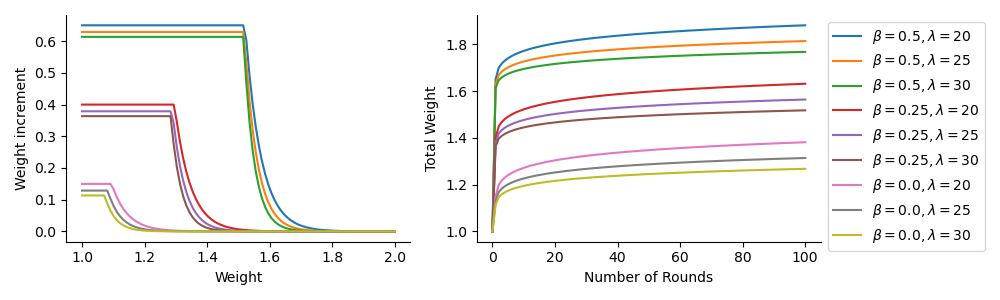
\includegraphics[width=0.85\textwidth]{images/plasticity.png}
    \caption{On the left we exhibit the plasticity increment, $\min\{\alpha , e^{\lambda (1 + \beta - w(t))} \}$, as a function of the weight; on the right is the total weight versus the number of rounds of training. Here, $\alpha = \beta + \log \lambda / \lambda$ as we assume in all of our proofs and experiments.}
    \label{fig:plasticity}
\end{figure}

\paragraph{Assemblies.} In this work, we will refer to sets of $k$ neurons in a single brain area as \emph{assemblies} when the internal synaptic weights of the set have been sufficently strengthened. We will also refer to the ``weight" from one assembly to another when we scale all the synapses between them by the same factor. A major result of previous work is that assemblies emerge naturally from the NEMO dynamical system\footnote{In fact, the assemblies obtained this way have additional properties, such as synapse density higher than the base synapse density $p$.}\cite{papadimitriou2020brain}; in this work, we take assemblies as a starting point for representing inputs and outputs to NEMO.

% \paragraph{Homeostasis.} Homeostasis happens over longer timescales. We abstract homeostasis at each neuron by rescaling its synaptic weights to maintain some semi-norm of its weight vectors, possibly specific to each area. While previously in NEMO only the $1$-norm of all weights was considered \cite{papadimitriou2020brain}, here we also consider top-$m$-norms of the weights from a single area. The top-$m$-norm of a vector is the sum of the $m$ absolute largest components, with the top-$1$-norm recovering the $\infty$-norm and the top-$n$-norm the $1$-norm. Thus, the update is
% \[w_{B, i} \gets \frac{m}{\|w_{B, i}\|_{(m)}} w_{B, i}\]
% where $w_{B, i}$ is the weight vector from area $B$ to neuron $i$ and $\|\cdot \|_{(m)}$ is the top-$m$-norm.


% Outline NEMO, with area-wide inhibition (interneurons), new top-$k$-norm homeostasis, and random perturbations to input (noisy neurons, or external influence). \mitro{include in this section that ``we sometimes consider settings where an  area $A$ contains a single, fixed assembly $I$ that fires as an input stimulus into other areas (and no neurons outside of $I$ in $A$ ever fire); in this case we'll call such an assembly an input assembly, and ignore its containing area / model only the $k$ neurons of the assembly and their synapses." (this is for ``I" below). Also we should briefly define the notion of total ``weight" from one set of neurons to another, i.e. sum of of all incoming synapses. }

\section{Computational Experiments}
\subsection{The assembly coin-flip}
%% mitro: the transition from 3 to 4.1 could be improved (but maybe it will become too long, in which case this is good as is). The issue is these "assemblies" crop up out of nowhere; where do they come from? 3 doesn't discuss how assemblies are engendered (but writing that up would take up a lot of space...l)
We first consider the situation where weights from some input assembly $I$ to assemblies $A_1, \ldots, A_m$ in area $S$ are increased (Figure \ref{fig:coinflip-schematic}). Then $I$ fires, while the activations of neurons in $S$ are perturbed by Gaussian noise; in subsequent rounds, only $S$ fires. A preliminary observation is that if any of $A_1, \ldots, A_m$ has sufficiently large weight from $I$, then after a few rounds of firing the set of firing neurons converges to one of $A_1, \ldots, A_m$. In every experiment in this section, we have $n=25000, k=500, p=0.1$, and the standard deviation of the noise is $5 \sqrt{kp}$.
% \mitro{Worth adding: if we also allow $I$ to fire in rounds $t > 1$, the set of firing neurons converges to an $A_i$ even faster (?). Could be footnote}

\begin{figure}[b]
    \centering
    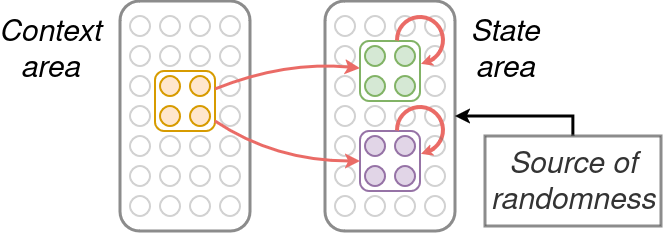
\includegraphics[width=0.7\linewidth]{images/assembly_coinflip_context.png}
    \caption{Choosing one of two assemblies to fire, based on context. The probability distribution depends on the weights of each assembly from the context (Theorem \ref{thm:coinflip}).}
    \label{fig:coinflip-schematic}
\end{figure}

In our first experiment (Figure \ref{fig:coinflip-exp}(a)), we fix a sample of the random graph, and measure how the probability that the firing neurons converge to $A_1$ changes as the weight from $I$ to $A_1$ is varied, while weights from $I$ to $A_2$ and $A_3$ are fixed (here at $2$). The internal weights of $A_1, A_2, A_3$ are set to $2$ as well. We repeat the process for $1000$ realizations of the random noise, and compute the empirical frequency that $A_1$ fires. We also plot the softmax function of the weights, where the rate parameter $\lambda$ is chosen empirically to minimize the error between the softmax and the empirical frequency (averaged over graphs). Qualitatively and empirically, this demonstrates that the probability distribution over assemblies is approximately a softmax of the incoming weights to the assemblies (see also Theorem \ref{thm:coinflip}).



\begin{figure}
    \centering
    \begin{subfigure}{0.3\textwidth}
    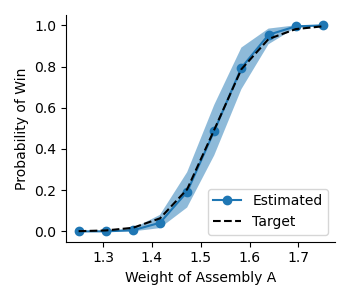
\includegraphics[width=\textwidth]{images/prob_vs_weight.png}
    \caption{}
    \end{subfigure}
    \hfill
    \begin{subfigure}{0.69\textwidth}
    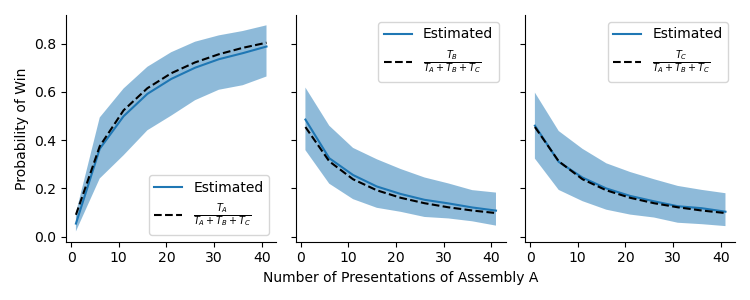
\includegraphics[width=\textwidth]{images/prob_vs_presentations.png}
    \caption{}
    \end{subfigure}
    \caption{Variation in the probability that assembly $A$ wins as its weight from the context assembly is varied, while the weights to $B$ and $C$ are held constant (and equal). On the left the weight is directly adjusted and compared against a best-fitting softmax function (dashed line); on the right all weights are updated incrementally according to a plasticity rule which approximately recovers the observed frequency (dashed line). Dark center line is the mean, while shaded area is the $[0.05, 0.95]$ quantile range, across 100 trials.}
    \label{fig:coinflip-exp}
\end{figure}

In the previous experiment, we directly set the synaptic weights between the input and output assemblies, and studied the resulting probability distribution (of the firing neurons converging to an output assembly). In other words, this shows how \emph{sample} a random variable, assuming its distribution has somehow already been learned and ``stored" in the synaptic weights. %In NEMO, weights can evolve only via the plasticity rule applied to concurrently firing neurons. 
However, the same neural representations of the outcomes of random variable $A$, namely the assemblies $A_i$, can be used to input \emph{observations} of the random variable during learning. It would be remarkable if, after presenting samples in this way, the probability distribution obtained by running the \emph{previous} experiment (for sampling) yields the empirical distribution seen during training (i.e., the probability the firing neurons converge to $A_i$ is the frequency with which $A_i$ was presented).

This motivates our second experiment (Figure \ref{fig:coinflip-exp}(b)), where we fix a random graph, and then present training samples to the model as follows: first fire $I$, and then $A_i$ repeatedly $T_i$ times. We then measure how the probability that each of $A_1, A_2, A_3$ fire changes as $T_1$ varies, with $T_2 = T_3 = 5$. We also plot the empirical frequency, $\frac{T_i}{T_1 + T_2 + T_3}$. The parameters of the plasticity rule are $\alpha = 0.63$, $\beta = 0.5$, and $\lambda = 26$. Remarkably, plasticity updates suffice to arrive at weights that sample from the empirical distribution! We refer the reader to Corollary \ref{cor:target} and Lemma \ref{lemma:plasticity} for a formal statement of this result and derivation of this plasticity rule.

Finally, to verify that the same plasticity rule suffices to learn distributions over various numbers of assemblies (outcomes), in Figure \ref{fig:inc-outcomes} compare the learned distribution as the number of assemblies that fired during training changes. Notably, a single plasticity rule approximately recovers the observed frequency, even when the number of outcomes is relatively large. In the first experiment (Figure \ref{fig:inc-outcomes}(a)) we vary the number of outcomes, while $A_1$ fires $5(m-1)$ times and $A_2, \ldots, A_m$ fire $5$ times during training; in the second (Figure \ref{fig:inc-outcomes}), $A_1$ fires $10$ times and $A_2, \ldots, A_m$ fire $5$ times. For both, we report the empirical frequency of $A_1$, estimated from $500$ samples over $100$ trials.

\begin{figure}[h]
    \centering
    \begin{subfigure}{0.35\linewidth}
        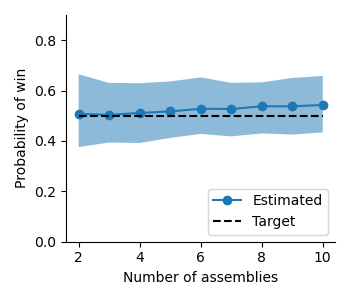
\includegraphics[width=\textwidth]{images/prob_vs_num_flat.png}
        \caption{}
    \end{subfigure}
    \begin{subfigure}{0.35\linewidth}
        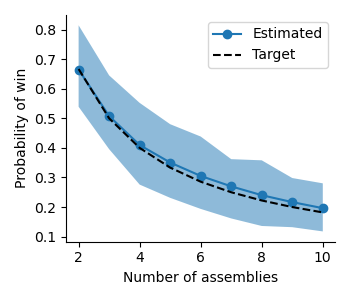
\includegraphics[width=\textwidth]{images/prob_vs_num_const.png}
        \caption{}
    \end{subfigure}
    \caption{Variation in the probability of an assembly winning, as the support of the training distribution grows to include more assemblies, under a plasticity rule that approximately recovers the training distribution. For two different sequences of distributions, we plot the empirical probability of assembly $A_1$ firing (blue dotted line) along with the target probability from the training distribution (black dashed). In (a) and (b) $A_2, \ldots, A_m$ fire $5$ times during training, for each $m=2,\ldots,10$, while in (a) $A_1$ fires $5(m-1)$ times and in (b) $A_1$ fires $10$ times for each $m$.}
    \label{fig:inc-outcomes}
\end{figure}

% However, the weights are not set directly. Rather, the plasticity rule incrementally adjusts each weight each time a pair of neighboring neurons fires concurrently. Hence, when the firing of one assembly ($I$ above) is followed by the firing of others at various frequencies, it is ultimately the plasticity rule (via its control of the weights) that determines what probability distribution this activity will induce. One desirable probability would simply be the identity -- i.e. the probability that the firing neurons converge to an assembly is the frequency with which that assembly fired.
% In our second experiment (Figure \ref{fig:coinflip-exp}(b)), with the graph again fixed, we ``learn'' the weights incrementally by firing $I$ followed by $A_i$ repeatedly $T_i$ times, with Hebbian plasticity in effect. We then measure how the probability that each of $A_1, A_2, A_3$ fire changes as $T_1$ varies, with $T_2 = T_3 = 5$. We also plot the empirical frequency, $\frac{T_i}{T_1 + T_2 + T_3}$. In both of these experiments, we have $n=25000, k=500, p=0.1$, and the standard deviation of the noise is $10 \sqrt{kp}$. The parameters of the plasticity rule are $\alpha = 0.4$, $\beta = 10$, and $\lambda = 13$. Refer to Corollary \ref{cor:target} and Lemma \ref{lemma:plasticity} for a formal statement of this result and derivation of this plasticity rule.

% \paragraph{Plasticity rule.} The plasticity rule used here and in the remainder of our simulations is
% % \[w_{ij}(t+1) = w_{ij}(t) + \frac{c}{\lambda} \frac{1 - \frac{kp}{m}}{\left(1-\frac{kp w_{ij}(t)}{kp w_{ij}(t) + m - kp}\right)^2} \exp\left(- \lambda \left(\frac{m w_{ij}(t)}{kp w_{ij}(t) + m - kp}-1\right)\right) \]
% \[w_{ij}(t+1) = w_{ij}(t) + \beta \exp\left(-\lambda w_{ij}(t)\right)\]
% each time neuron $i$ fires followed by neuron $j$, where $w_{ij}$ is the weight from $i$ to $j$. The parameters of the rule are $\beta$ and $\lambda$. Note that this rule is Hebbian and involves only synapse-local information. This rule can be derived as follows (see Lemma \ref{lem:plasticity} for the rigorous claim).
% Specifically, from the observation that the distribution over assemblies is the softmax of the weights, it is clear that we will have approximately proportional sampling when
% $e^{\lambda w_i} = c T_i$ for each $i=1,\ldots, l$,
% where $\lambda$ is the rate of the softmax, $c$ is a constant, $w_i$ is the weight to assembly $A_i$ and $T_i$ is the number of times $A_i$ fired during training. This in turn gives $$
% By choosing $c = \beta \lambda e^{\lambda}$, we obtain $w(t) = 1 + \frac{\beta}{\lambda} \log t$ where $\hat w(t)$ is the weight after seeing an assembly fire $t$ times and applying homeostasis. Using the local estimate for the top-$m$-norm $w(t) \cdot kp + m - kp$, we obtain
% \[w(t) = \frac{m - kp}{m - (1 + \lambda^{-1} \log t)kp} (1 + \lambda^{-1} \log t)\]
% and differentiating this function in $t$ gives the plasticity rule.

\subsection{Scaling} 
One important observation about the assembly coinflip is that a substantially higher scale is required for the phenomenon to emerge compared to previous work in NEMO \cite{dabagia2022assemblies, dabagia2024computation} -- say, $k=500$ versus $k=30$. Accordingly, we examine this scaling phenomenon quantitatively in Figure \ref{fig:inc-size}. For simplicity we consider the case where the target distribution over assemblies $A$ and $B$ is uniform, so the weights to each are the same -- here, $2$. For each choice of cap size ($k$) we sample $20$ connectivity graphs, increase the weights, and estimate the resulting distribution from $500$ samples. We then plot the resulting absolute deviation of $A$ firing from $1/2$. Notably, the error does not reach $0$, even for very large $k$, but nor do we expect it to, since the maximum deviation of $20$ $(500, 1/2)$ binomial random variables is roughly $0.1$ in expectation (i.e. if the learned distribution were completely unbiased, and the only error was due to sampling).

\begin{figure}[h]
    \centering
    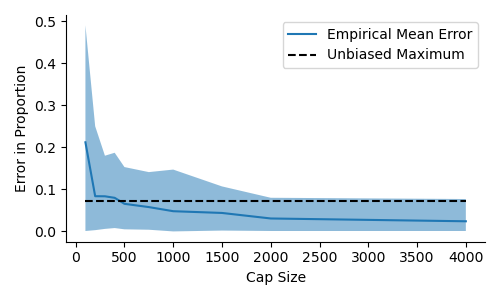
\includegraphics[width=0.5\textwidth]{images/error_vs_cap_size.png}
    \caption{Variation in the error of the learned distribution over two assemblies as the cap size increases. For each of $20$ trials, a new connectivity graph was sampled, the assemblies $A$ and $B$ were made to fire exactly the same number of times, and the resulting distribution was estimated from $500$ samples. The absolute deviation of the frequency with which $A$ won from $1/2$ was recorded for each trial. The dark center line is the mean of this error over trials, the shaded area is the range, and the dashed line is the \emph{expected maximum} if the samples were truly unbiased (i.e. the probability that $A$ comes to fire is exactly $1/2$). }
    \label{fig:inc-size}
\end{figure}


\subsection{Learning Markov chains}
Next, we examine how accurately the transitions of a Markov chain can be learned from a stream of samples, using the basic mechanism demonstrated above (see Corollary \ref{cor:markovchain} for the theoretical formulation of this result). We assume that there ares area $A$ and $B$ which contain an assembly $A_s$, $B_s$ for each state $s$ of the Markov chain (see Figure \ref{fig:mc-schematic}). The areas ``lazily'' alternate firing, so that $A$ fires once while $B$ is inhibited, then $B$ fires $10$ times while $A$ is inhibited, then $A$ fires again once, and so forth.
There are connections in both directions between $A$ and $B$, initially all $1$. Internally, weights within each $A_s$ and $B_{s}$ are strengthened by a factor of $2$.

\begin{figure}
    \centering
    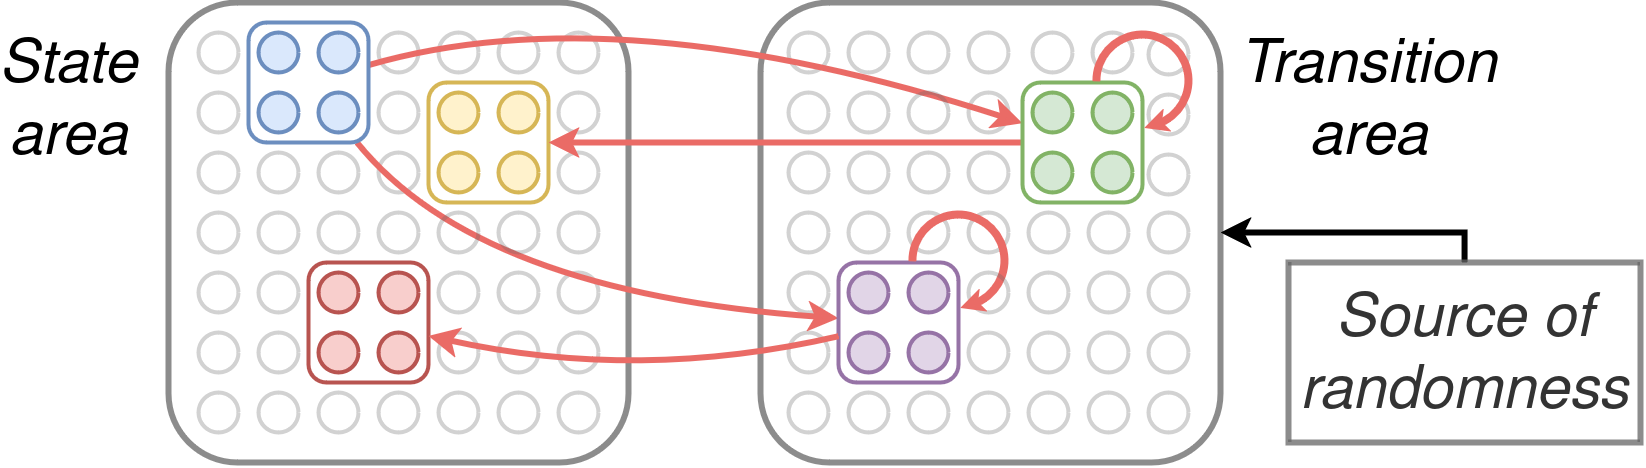
\includegraphics[width=0.9\linewidth]{images/assembly_markov_chain.png}
    \caption{Realizing the transitions of a Markov chain using assemblies (Corollary \ref{cor:markovchain}). Both the state and transition areas contain an assembly for each state. Assemblies in the state area are connected to transition assemblies, with the synaptic weights from a state assembly to the transition assemblies encoding the probability of transitioning to those states.}
    \label{fig:mc-schematic}
\end{figure}

\begin{figure}[b]
    \centering
    \begin{subfigure}{0.49\textwidth}
        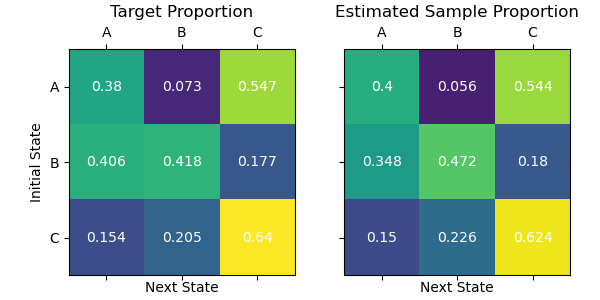
\includegraphics[width=\textwidth]{images/dense_trans_mat.png}
        \caption{}
    \end{subfigure}
    \hfill
    \begin{subfigure}{0.49\textwidth}
        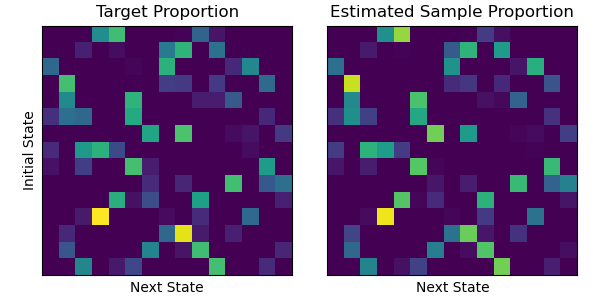
\includegraphics[width=\textwidth]{images/sparse_trans_mat.png}
        \caption{}
    \end{subfigure}
    \caption{We compare an estimate of the transition matrix learned by the model from a stream of samples from a Markov chain with the true transition matrix. This model is trained by presenting sequences of states, sampled from a ground-truth Markov chain, and then firing the appropriate state and transition assemblies in an alternating fashion, with the weights updated by the appropriate Hebbian rule. In both (a) and (b) the left is the ground truth transition matrix (which training samples were generated from) and the right is estimated empirical transition matrix. In (a) we show a chain with a dense transition graph, and in (b) a chain with a sparse transition graph.}
    \label{fig:mc-exp}
\end{figure}

The basic idea of the Markov model is to treat $A$ as the ``context'' area in the coinflip model, and $B$ as the ``state'' area, so that assemblies in $B$ are outcomes with probability conditional on the assembly firing in $A$. The model is trained by presenting a stream of states sampled from the target Markov chain, say $s_1,\ldots,s_t, \ldots$. Training proceeds by firing $A_{s_1}$, followed by $B_{s_2}$, followed by $A_{s_2}$ and so on. In Figure \ref{fig:mc-exp}, the training sequences had length $100 \cdot \# \text{ of states}$. At test time, we sample from the Markov chain by simply firing an initial state, and then observing the activity in area $A$ every $10$ rounds. To estimate the transition probabilties, for each state, we sample $1000$ realizations of random noise and record the empirical frequency of each transition. In Figure \ref{fig:mc-exp} we display the results of learning two chains: one has three states and every transition has positive probability, and the other has $15$ states but each state transitions to only five states with positive probability. For each instance, we display the empirical transition matrix estimated from samples alongside the ground-truth transition matrix from which the training examples were sampled. Here, $n=25000, k=500, p=0.1$, and the noise has standard deviation $5 \sqrt{kp}$, while the plasticity parameters are $\alpha = 0.63$, $\beta = 0.5$, and $\lambda = 26$.

\subsection{Statistical learning of language}
Our final experiment applies the probabilistic machinery described so far to construct a primitive model of language (Figure \ref{fig:trigram}). Consider a corpus of language, which is a set of strings comprised of tokens from a lexicon $\mathcal T$. We suppose there exist brain areas $A, B, C$, with connections from $A$ to $B$, $B$ to $A$ and $C$, and $C$ to $A$. The areas contain assemblies $A_\tau, B_\tau, C_\tau$ for each token $\tau \in \mathcal T$; the firing of $A_\tau$ represents token $\tau$ being presented to the model. Internal connections of these assemblies are assumed to be strengthened, and connections from $A_\tau$ to $B_\tau$ and $B_\tau$ to $C_\tau$, but otherwise no weight changes have occurred. Training then proceeds as follows: For a string of tokens $\tau_1, \tau_2, \ldots,$ we fire $A_{\tau_1}, A_{\tau_2}, \ldots$. As this activity propagates to areas $B$ and $C$, the result is strengthening the connections to $A_{\tau_t}$ from $B_{\tau_{t-1}}$ and $C_{\tau_{t-2}}$. Sampling then occurs in area $A$: To sample a third token in the trigram $(\tau_1, \tau_2, \cdot)$, $B_{\tau_2}$ and $C_{\tau_1}$ fire simultaneously, then $A$ is allowed to fire $10$ times, while connections from $A$ to $B$ and from $B$ to $C$ are inhibited, then $A$ is inhibited while inter-areal connections are again enabled. After this process concludes, for some $\tau_3$ we should have $B_{\tau_3}$ along with $C_{\tau_2}$ firing, so sampling may repeat to generate a stream of tokens. Here, we take $n=100,000, k=500, p=0.1$, with plasticity parameters $\alpha=0.63, \beta=0.5, \lambda=60$. The model was trained by presenting the entire corpus $5$ times. We emphasize that no settings or changes were made to NEMO to specialize to the data or output. 

\begin{figure}[t]
    \centering
    \begin{subfigure}{0.4\textwidth}
        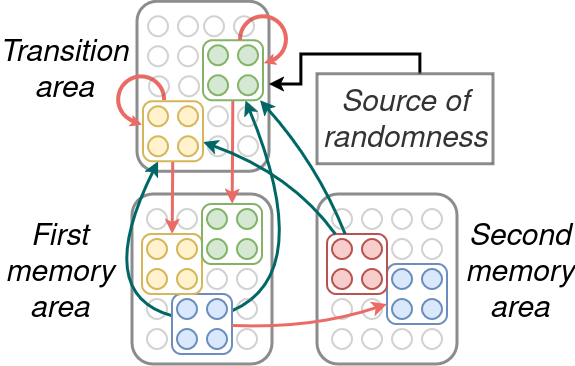
\includegraphics[width=\textwidth]{images/assembly_trigram.png}
        \caption{}
    \end{subfigure}
    \hfill
    \begin{subfigure}{0.59\textwidth}
        \centering
        \begin{tabular}{p{0.95\textwidth}}
            \texttt{the owl and the pussycat went to sea in a wood a piggy wig stood with a ring. they took some honey and plenty of money wrapped up in a beautiful pea green boat. they took some honey and plenty of money wrapped up in a wood a piggy wig stood with a ring. they took it away and were married next day by the light of the moon.}
        \end{tabular}
        \caption{}
    \end{subfigure}
    \caption{In (a), we exhibit a schematic of a simple trigram model of language within NEMO. In (b), we show an example string generated after training the model with the text of the poem ``The Owl and the Pussy-Cat'' by Edward Lear, where each word and punctuation mark is a token. The poem contains 109 tokens comprising 182 unique trigrams.}
    \label{fig:trigram}
\end{figure}



% with connections from $W$ to $X$ and $A$, from $X$ to $Y$ and $A$, from $Y$ to $A$, and from $A$ to $W$. $W, X, Y$ contain assemblies $W_\tau, X_\tau, Y_\tau$ for each token $\tau \in \mathcal T$; the firing of $W_\tau$ represents token $\tau$ being presented to the model. Internal connections of $X_\tau, Y_\tau$ are assumed to be strengthened, and connections from $W_\tau$ to $X_\tau$ and from $X_\tau$ to $Y_\tau$, but otherwise no weight changes have occurred. Training then proceeds as follows: For each tuple $t = (\tau_1, \tau_2, \tau_3)$ which is present in the corpus, we create an assembly $A_t$ by firing $W_{\tau_1}, X_{\tau_2}, Y_{\tau_3}$ together a few times, which additionally strengthens the connection from $A_t$ to $W_{\tau_1}$. We then simply present the corpus to the model repeatedly, by firing the appropriate sequence of assemblies $W_{\tau_1}, W_{\tau_2},\ldots$ every other round, such that $\{W, X, Y\}$ and $A$ alternate firing. To sample from the model, we assume that each time $\{W, X, Y\}$ fire, then $A$ fires $10$ times, and present an initial sequence of tokens. When $X_{\tau_2}, Y_{\tau_3}$ fire together, this triggers sampling to occur in $A$ to select an assembly $A_t$ to fire corresponding to $t = (\tau_1, \tau_2, \tau_3)$ for some assembly $\tau_1$. This then triggers $W_{\tau_1}$ to fire, followed by $X_{\tau_1}, Y_{\tau_2}$, and sampling may repeat.


\section{Theoretical Results}

\paragraph{Outline} The presentation of our theoretical results follows the development of the experiments in the previous section. We first establish the basic ingredient of our neuronal-level statistical learner -- randomly choosing one assembly out of a set of possible ``outcome'' assemblies to fire, according to a probability distribution which depends on the weights from the context assembly to the outcome assemblies. This sampling procedure is driven by random noise, which we model here as an i.i.d. perturbation to each neuron's activation. The formal claim that this behavior provably occurs in NEMO (when the set of outcomes has size 2) is the content of Theorem \ref{thm:coinflip}. This gives the distribution as a function of the weights; in Corollary \ref{cor:target}, we determine the weights necessary to achieve a target distribution. Lemma \ref{lemma:plasticity} is the formal claim that the plasticity rule used in our experiments incrementally adjusts the weights during training to ensure that the probability that an assembly fires after training replicates its observed frequency in the training phase. Finally, Corollary \ref{cor:markovchain} uses this mechanism as the building block of a more complex model, namely the simulation of a restricted class of Markov chains using assemblies.

We now proceed with the statement of Theorem \ref{thm:coinflip}. At a high level, this theorem gives sufficient conditions for the parameters of the model such that the distribution of over outcome assemblies is close to a distribution which depends only on the weights of the outcome assemblies (Figure \ref{fig:coinflip-schematic}). It is worth noting that there are two sources of randomness in play: One is the random graph which determines connectivity, and the other arises from the noise model's perturbations to neuronal activations. For our purposes, it is desirable that the realized distribution over outcomes be nearly independent of the random graph. Since complete independence is impossible, we settle for high probability, so that the probability that the realized distribution deviates significantly from a distribution genuinely independent of the connectivity goes to zero as $n$ (the number of neurons) goes to $\infty$.

% The first basic ingredient of our neuronal-level statistical learner is choosing one assembly out of a set of ``outcome'' assemblies to fire (Figure \ref{fig:coinflip-schematic}), so that the probability distribution over outcome assemblies is approximately determined by the weights from a context assembly to the outcome assembly. The formal claim that this behavior provably occurs in NEMO (when the set of outcomes has size 2) is the content of Theorem \ref{thm:coinflip}.
% \begin{theorem}[\textbf{Conditional Coin-Flipping}] \label{thm:coinflip}
% Let $I, M$ be brain areas, with $I_0 \subseteq I, A, B \subseteq M$ all disjoint sets of size $k$, such that weights from $I_0$ to $A$ (resp. $B$) are strengthened by a factor of $w_A$ (resp. $w_B$), and weights within $A$ (resp. $B$) are strengthened by a factor of $w$, and no other weights from $I_0$ to $M$ are strengthened. Suppose that $I_0$ fires once, and the resulting total inputs to neurons in $M$ are perturbed by i.i.d. $\mathcal N(\mu, \sigma^2 kp)$ random variables. Suppose that $p \ge \frac{\log^2 n}{k}$, $w_A, w_B \ge 1 + 4 \sigma \sqrt{\frac{\log n}{kp}}$, and $w \ge 1 + 2 \sqrt{\frac{\log n}{kp}}$. Let $C_t$ denote the set of neurons firing in $M$ after $t$ rounds.
% Then there exists some $\lambda = \lambda(n, k, p)$ such that for all $t \ge \frac{\log k}{\log(kp)}$,
% \begin{align*}
%     \left|\Pr(C_t = A | \mathcal G) - \Phi\left(\lambda \frac{w_A - w_B}{\sigma}\right) \right| &= o(1)\\
%     \left|\Pr(C_t = B | \mathcal G) - \Phi\left(\lambda \frac{w_B - w_A}{\sigma}\right) \right| &= o(1)
% \end{align*}
% with high probability over the realization of the random graph, $\mathcal G$, as $n, \sigma \to \infty$
% \end{theorem}

\begin{theorem}[\textbf{Conditional Coin-Flipping}] \label{thm:coinflip}
    Consider NEMO brain areas $I$ and $M$, with a context set $I_0 \subseteq I$ and outcome sets $A, B \subseteq M$, all disjoint and of size $k$. Let the connections from $I_0$ to $A$ (resp. $B$) be strengthened by a factor of $w_A$ (resp. $w_B$), and the connections from $A$ to $A$ and from $B$ to $B$ be strengthened by a factor of $w_R$, and all other connections from $I_0 \cup A \cup B$ to $M$ have weight $1$. Suppose that $I_0$ fires once, and the total inputs to neurons in $M$ are perturbed by i.i.d. $\mathcal N(\mu, \sigma^2 kp)$ random variables. 
    
    Let $C_t$ denote the set of $k$ neurons firing in $M$ after $t$ rounds. Then there exist $p, w_0, w_R, \sigma, \tau, t_0$ such that if $w_A, w_B \ge w_0$, for all $t \ge t_0$ we have
    \begin{align*}
        \left|\Pr(C_t = A | \mathcal G) - \Phi\left( \frac{w_A - w_B}{\tau}\right) \right| = o(1),\hspace{1cm} \left|\Pr(C_t = B | \mathcal G) - \Phi\left(\frac{w_B - w_A}{\tau}\right) \right| &= o(1)
    \end{align*} with high probability over the random graph $\mathcal G$ as $n \to \infty$. Here, $\Phi$ is the Gaussian CDF\footnote{It is worth noting that the appearance of the Gaussian CDF here is \emph{not} due to the normal distribution of the noise, but rather because under fairly general assumptions sample quantiles are asymptotically normally distributed.}.
\end{theorem}

The upshot of Theorem \ref{thm:coinflip} is that there is an explicit function of the weights only, which does not depend on the actual realization of the underlying graph (only on the parameters of the model), so that the actual probability distribution over outcomes is very close to this function.
A natural question is whether we can set the weights in such a way that some target probability distribution is realized. 
% Moreover, in NEMO the weights $w_A$ and $w_B$ are not set explicitly, but rather adjusted incrementally by Hebbian plasticity. So, the choice of plasticity rule determines the probability distribution over $A$ and $B$, as a function of the number of times that each fires. 
We first characterize in the next corollary the weights necessary to achieve a certain probability distribution on the eventual firing of $A$ or $B$.
% The next corollary establishes what the weights should be to achieve proportional sampling -- when the probability that $A$ fires is proportional to the number of times it was observed to fire.

\begin{corollary} \label{cor:target}
    Under the assumptions of Theorem \ref{thm:coinflip}, there exist $c, \lambda > 0$ such that, if 
    \begin{align*}
        \left|w_A - \frac{\log c T_A}{\lambda}\right| \le \frac{1}{50\lambda}, \hspace{2cm}
        \left|w_B - \frac{\log c T_B}{\lambda}\right| \le \frac{1}{50\lambda}
    \end{align*}
    then for all $t \ge t_0$ we have
    \[\left|\Pr(C_t = A | \mathcal G) - \frac{T_A}{T_A + T_B} \right| < 1/ 25 + o(1)\]
\end{corollary}
The essence of this result is just showing that the Gaussian CDF $\Phi(x)$ is close to the logistic function ($2$-dimensional softmax), $\frac{e^{\lambda x}}{1 + e^{\lambda x}}$, for appropriate choice of $\lambda$.

We now establish a plasticity rule which, through the dynamics of NEMO, induces weights through training such that the induced probability distribution approximates the observed frequency.

% Specifically, from the observation that the distribution over assemblies is the softmax of the weights, it is clear that we will have approximately proportional sampling when
% $e^{\lambda w_i} = c T_i$ for each $i=1,\ldots, l$,
% where $\lambda$ is the rate of the softmax, $c$ is a constant, $w_i$ is the weight to assembly $A_i$ and $T_i$ is the number of times $A_i$ fired during training. This in turn gives $$
% By choosing $c = \beta \lambda e^{\lambda}$, we obtain $w(t) = 1 + \frac{\beta}{\lambda} \log t$ where $\hat w(t)$ is the weight after seeing an assembly fire $t$ times and applying homeostasis. Using the local estimate for the top-$m$-norm $w(t) \cdot kp + m - kp$, we obtain
% \[w(t) = \frac{m - kp}{m - (1 + \lambda^{-1} \log t)kp} (1 + \lambda^{-1} \log t)\]
% and differentiating this function in $t$ gives the plasticity rule.

\begin{lemma} \label{lemma:plasticity}
    Under the assumptions of Theorem \ref{thm:coinflip}, suppose that the weight update is
    \[w_{ij}(t+1) = w_{ij}(t) + \max\{\alpha, e^{\lambda (1 + \beta - w_{ij}(t))}\}\]
    when neuron $j$ fired on round $t$ and neuron $i$ fired on round $t+1$, and $w_{ij}(t)$ is the weight of the synapse from $j$ to $i$ on round $t$. Suppose that $A$ fires after $I_0$ $T_A$ times, and $B$ fires after $I_0$ $T_B$ times. Then there exists $T_0, \alpha, \beta, \lambda$ such that for $T_A, T_B \ge T_0$,
    \begin{align*}
        \left|\Pr(C_t = A \cond \mathcal G) - \frac{T_A}{T_A + T_B}\right| < \frac{1}{25} + o(1).
    \end{align*}
\end{lemma}
Note that the plasticity rule is still Hebbian, and completely synapse-local; what is specified is only the magnitude of the change in weight, as a function of the current weight.  This rule is a natural approximation of the ``target'' weights for proportional sampling given in Corollary \ref{cor:target}, as follows. For $t=0$, we have $w(0) = 1$ and the target $w(1) = \lambda^{-1} \log c$, so the incremental change is simply $w(1) - w(0) = \lambda^{-1} \log c$. For $t \ge 1$, the increment is 
\[w(t+1) - w(t) = \frac{\log(c(t+1)) - \log (ct)}{\lambda} = \frac{\log(1+1/t)}{\lambda}.\]
 We use the approximation $\log(1 + 1/t) \approx 1/t$, and then use the assumption that $t = e^{\lambda w(t)} / c$ (which is exactly true for the target weight) to get $w(t+1) - w(t) = \frac{c}{\lambda} e^{-\lambda w(t)}$. We take $c = \lambda e^{\lambda(1 + \beta)}$ and set $\alpha = \beta + \lambda^{-1} \log( \lambda)$ to recover the parameterization of the rule in the lemma.

Using the above result, we show rigorously that a finite, stationary Markov chain with out-degree at most 2 can be simulated in NEMO.

\begin{corollary}[Markov Chain] \label{cor:markovchain} Consider a Markov chain with states $s =1,\ldots,m$, such that the transition probabilities from $s$ to state $\rho(s, i)$ is $p_{s, i}\ge0$ for $i=1,2$ and $0$ for all other states. Consider distinct brain areas $A$ and $B$, with disjoint state sets $A_s \subseteq A, B_s \subseteq B$ for $s=1, \ldots, m$. Suppose that when $A$ fires $B$ fires for $t$ rounds while $A$ is inhibited, then $B$ is inhibited and $A$ is permitted to fire. Furthermore, suppose for each $s=1,\ldots, m$, $i=1,2$, weights from $A_s$ to $B_{\rho(s, i)}$ are strengthened by a factor of $\frac{1}{\lambda}\log(c \cdot p_{s, i}) + 1$, and weights from $B_{s}$ to $A_{s} \cup B_s$ are strengthened by $w_R$. Then there exist $p, c, \lambda, \sigma, t$ such that for all $s=1,\ldots,m$, $i=1,2$, if $A_s$ fires, the probability that $A_{\rho(s, i)}$ fires $t+1$ rounds later deviates from $p_{s, i}$ by no more than $1/50$, w.h.p. as $n \to \infty$.
\end{corollary}
In the notation of the corollary, this means that a model configured as above approximates the Markov chain with states $\{1, \ldots, m\}$, and with transition probability from state $s$ to state $\rho(s, i)$ of $p_{s, i}$. Using the plasticity rule in Lemma \ref{lemma:plasticity}, the transition probabilities can be learned from a sequence $s_1, s_2, \ldots$ sampled from the target Markov chain by firing the assemblies $A_{s_1}, B_{s_2}, A_{s_2}, B_{s_2}, \ldots$. Furthermore, out-degree 2 Markov chains are general in the following sense:

\begin{remark}
Consider a Markov chain with states $[m]$ and transition probability $p_{i, j}$ from state $i$ to state $j$. Then there exists a Markov chain $(X_t)$ with states $[m] \times [m-1]$ and out-degree $2$ such that
\[\Pr(X_{t + \max\{j, m-1\}} = j \cond X_t = i) = p_{i, j}.\]
\end{remark}
Intuitively, this construction reduces a single random choice of one item out of many to a sequence of binary choices, whether to choose a particular item or discard it and repeat with the smaller set. In terms of the transition graph of a Markov chain, it replaces each random transition with a binary tree of transitions, whose leaf vertices correspond to states in the original chain.

% Finally, by combining the above results, we show rigorously that a finite, stationary Markov chain can be simulated in NEMO. Moreover, if the out-degree of every state in the Markov chain is at most $2$ the simulation can be configured simply by presenting samples from the chain.

% \begin{corollary}[Markov Chain] \label{cor:markovchain}Explain how with assemblies for each state, and associated transition in assemblies in a separate area, we can simulate the transitions of a Markov chain.
% \end{corollary}

\paragraph{The noise assumption.}
In our experiments and proofs, we have assumed that neuronal activations are perturbed by i.i.d. Gaussian noise. Due to the Central Limit Theorem, this is a reasonable way to abstractly model the contribution of many small independent sources of uncertainty. In particular, one can explicitly model the source of randomness in the setting of Theorem \ref{thm:coinflip} by adding an additional area $R$ of size $\sigma^2 n$ with connections to area $A$, and assume that the only randomness is that a \emph{random set} of $k$ neurons fires in $R$. The resulting perturbations to the activations of neurons in $A$ will be independent, identically-distributed binomial $(\sigma^2 n, p)$ random variables, which under the CLT converge in distribution to $\mathcal N(\sigma^2 np, \sigma^2 np(1-p))$ with appropriate normalization.


\section{Proofs}
The proof of Theorem \ref{thm:coinflip} consists of showing that $A$ obtains a decent advantage on the first round using Lemma \ref{lemma:first-round} with the specified probability that $A$ wins altogether, and then showing that this initial lead will quickly grow to activate the entire assembly using Lemma \ref{lemma:conv-w-advantage}.
\begin{proof}[Proof of Theorem \ref{thm:coinflip}]
    First, WLOG, assume that $\mu = 0$. Let $X_i(0)$ denote the input to neuron $i$ when $I_0$ fires, and $Y_i \sim \mathcal N(0, \sigma^2 kp)$ denote the random perturbations; then we have
    \[X_i = \begin{cases} w_A \cdot e(I_0, i) + Y_i & i \in A\\
    w_B \cdot e(I_0, i) + Y_i & i \in B\\
    e(I_0, i) + Y_i & \text{o.w.}
    \end{cases}\]
    We will first establish that $C_t \subseteq A \cup B$ for all $t \ge 0$ w.h.p. by induction. For the base case, note that w.h.p. for all $i \not\in A \cup B$, we have $e(I_0, i) \le kp + \sqrt{3kp \log n}$ by the Chernoff bound; likewise, $Y_i \le \sigma \sqrt{3kp\log n}$. Hence,
    \[X_i \le kp + \sigma \sqrt{3 kp \log n} + o(kp).\]
    On the other hand, for all $i \in A \cup B$, we have
    \[X_i \ge \min\{w_A, w_B\} (1-o(1)) kp - \sigma \sqrt{3 kp \log n} \ge kp + \sigma \sqrt{3 kp \log n} + o(1) \ge \max_{j \not\in A \cup B}X_j\]
    for all sufficiently large $n, \sigma$. Hence, w.h.p. $C_0 \subseteq A \cup B$. Now, suppose that $C_t \subseteq A \cup B$. WLOG, suppose that $|C_t \cap A| \ge k/2$. Then for $i \in A$, we have
    \[X_i(t+1) \ge (1 + w) kp / 2 - o(1) \ge kp + o(1) = \max_{j \not\in A \cup B} X_j(t+1)\]
    for all sufficiently large $n$ w.h.p. Hence, every neuron in $A$ has larger input than every neuron outside of $A \cup B$, and so $C_{t+1} \subseteq A \cup B$. By the principle of induction, it follows that $C_t \subseteq A \cup B$ for all $t \ge 0$.

    Now, let $T_0$ be the median of $\{X_i(0) \colon i \in A \cup B\}$, and note that $i \in C_0$ if and only if $X_i(0) \ge T_0$. By Lemma \ref{lemma:first-round}, we have
    \begin{align*}
        \Pr(|C_0 \cap A| &\ge k/2 + \sqrt{k / \log k} \cond \mathcal G) \ge \Phi\left(\lambda \frac{k\sqrt{p}}{\sigma}(w_A - w_B)\right)\\
        \Pr(|C_0 \cap B| &\ge k/2 + \sqrt{k / \log k} \cond \mathcal G) \ge \Phi\left(\lambda \frac{k\sqrt{p}}{\sigma}(w_B - w_A)\right)
    \end{align*} Now, suppose that $ k - |C_t \cap A| \le \sqrt{k / \log k}$. Since $\sqrt{k / \log k} \ge 6 p^{-1}$,  by Lemma \ref{lemma:conv-w-advantage}, we will have 
    \[|C_{t+1} \cap A| \ge k/2 + \max\{k/2, \frac{\sqrt{kp}}{6}  (|C_t \cap A| - k/2)\}\]
    w.p. at least $1 - \exp\left(-(|C_t \cap A| - k/2)^2 p\right)$.
    Thus, if $|C_0 \cap A| \ge k/2 + \sqrt{k / \log k}$, then for all $t \ge 1$ we have
    \[|C_t \cap A| \ge k/2 + \max\{k/2, \left(\sqrt{kp}{6} \right)^t \sqrt{k / \log k}\}\]
    w.p. $1- o(1)$, and so after $t_0 = O(\log k / \log (kp))$ rounds, we must have $|C_{t_0} \cap A| = k$ w.h.p. A similar argument holds for $B$.
\end{proof}

\begin{proof}[Proof Sketch of Corollary \ref{cor:target}]
    One can verify (even numerically) that
    \[\sup_{x \in \R}\left|\frac{e^{1.6x}}{1 + e^{1.6x}} - \Phi(x)\right| < \frac{1}{50}.\]
    In particular, for $x = \frac{(w_A-w_B)}{\tau}$, and setting $\lambda = 1.6 / \tau$, we have
    \[ \frac{e^{1.6x}}{1+e^{1.6x}} = \frac{e^{1.6 w_A / \tau}}{e^{1.6 w_A / \tau}+ e^{1.6 w_B / \tau}} = \frac{e^{\lambda w_A}}{e^{\lambda w_A} + e^{\lambda w_B}} \]
    Now, for settings of $w_A$ and $w_B$ that satisfy the corollary conditions,
    \[\frac{e^{\lambda w_A}}{e^{\lambda w_A} + e^{\lambda w_B}} \approx \frac{c T_A}{cT_A + cT_B} \approx \frac{T_A}{T_A + T_B}\]
    where $\approx$ denotes an absolute difference of $o(1)$, and so
    \[\left|\Phi\left(\frac{w_A - w_B}{\tau}\right) - \frac{T_A}{T_A + T_B}\right| < 1/ 50 + o(1).\]
    We then take $c$ and $T_0$ large enough to ensure the condition on $w_0$ in Theorem \ref{thm:coinflip} is satisfied.
\end{proof}

\begin{proof}[Proof Sketch of Lemma \ref{lemma:plasticity}]
    We first note that for $\alpha = \beta + \lambda^{-1} \log(\lambda)$, one has $w(1) = \lambda^{-1}\log(c \cdot 1)$ for $c = \lambda e^{\lambda(1 + \beta)}$. 
    The substance of the proof is showing that for all $t \ge 2$, we have
    \[\frac{\log (c t)}{\lambda} \le w(t) \le \frac{\log (c(t + \log t))}{\lambda}.\]
    It is readily verified that $w(t)$ satisfying the above also meets the conditions of Corollary \ref{cor:target} and hence the desired probabilities obtain.
    The above claim reduces to showing that the recurrence relation
    \[x_{n+1} = x_n + e^{-x_n} \hspace{2cm} x_1 = 0\]
    satisfies $\log n \le x_n \le \log(n + \log n)$. This can be verified by induction; clearly it holds for $n=1$. For $n \ge 2$, we have the lower bound
    \[x_{n+1} = x_n + e^{-x_n} \ge \log n + \frac{1}{n} \ge \log (n+1).\]
    For the upper bound, it can be verified that the function 
    \[f(x) = \log(x + \log x) + \frac{1}{x + \log x} - \log(x+1 + \log(x+1))\]
    has a single extremum, at which it is positive, and since $f(1) = 0$ and $\lim_{x \to \infty}f(x) = 0$ the inequality $x_{n+1} \le \log(n+1 + \log(n+1))$ holds.
\end{proof}

\begin{proof}[Proof Sketch of Corollary \ref{cor:markovchain}]
    For each $s=1,\ldots,m$, Corollary \ref{cor:target} asserts that this choice of weights will ensure that when $A_s$ fires, the probability that $B_{\rho(s, i)}$ fires will be $p_{s, i} \pm 1/50$. For sufficiently large $w_R$, when $B_{\rho(s, i)}$ fires $A_{\rho(s, i)}$ will fire immediately after. So, by choosing $t$ larger than $t_0$ in Theorem \ref{thm:coinflip} we can ensure that the entirety of $B_{\rho(s, i)}$ fires when $A$ becomes disinhibited, so the probability that $A_{\rho(s, i)}$ fires in area $A$ $t$ rounds after $A_s$ is very nearly $p_{s, i}$.  
\end{proof}

\begin{lemma} \label{lemma:conv-w-advantage}   For $m \in [n]$, let $X_1, \ldots, X_n$ be i.i.d. $(m, p)$ binomial random variables, with $X_{(i)}$ their $i$th order statistic. Let $\Delta = |m - n/2|$ and set $k = \max\{\lfloor n/2 + \frac{\sqrt{np}}{6} \cdot \Delta \rfloor, n\}$. Then the following hold:
    \begin{enumerate}
        \item For $m \ge n /2 + 6p^{-1}$, we have
        \[\Pr(X_{(n-k)} \le np / 2) \le e^{-\Omega(\Delta^2 p)}\]
        \item For $m \le n /2 - 6p^{-1}$, we have
        \[\Pr(X_{(k)} \ge np / 2) \le e^{-\Omega(\Delta^2 p)}\]
    \end{enumerate}    
\end{lemma}

\begin{proof}
    First, if $\Delta \ge \sqrt{4 n \log n}$, then the Chernoff bound gives
    \[\Pr(X_1 \le np / 2) \le \exp\left(-\frac{4 \log n}{1 + 2 \epsilon}\right) \le \frac{1}{n^2}\]
    and so by the union bound we have $X_{(1)} > np/2$ w.p. $1 - 1/n$. For $\Delta < \sqrt{4n \log n}$,
    set
    \[Y = \sum_{i=1}^n \1_{\{X_i > np / 2\}}\]
    and note that $Y$ is a $(n, q_m)$-binomial random variable, where
    \[q_m = \Pr(X_1 > np / 2)\]
    Moreover,
    \[\Pr(X_{(n-k)} \le np / 2) = \Pr(Y \le k) \le \exp\left(-\frac{(n q_m - k)^2}{2n q_m}\right)\]
    via the Chernoff bound. Then using the Berry-Esseen theorem,
    \[1 - q_m = \Pr(X_1 \le np / 2) \le \Phi\left( -\frac{\Delta p}{\sqrt{mp(1-p)}}\right) + \frac{1}{2\sqrt{m p (1-p)}}\]
    where $\Phi \colon \R \to [0, 1]$ is the normal CDF. By Taylor's theorem, there exists $t \in [0, \Delta p]$ such that
    \[\Phi\left( -\frac{\Delta p}{\sqrt{mp(1-p)}}\right) = \Phi(0) - \frac{\Delta p}{\sqrt{mp(1-p)}} \cdot \phi \left(\frac{t}{\sqrt{mp(1-p)}}\right)\]
    where $\phi \colon \R \to \R$ is the normal PDF.
    Noting that $\phi$ is monotone decreasing for $t \ge 0$, we have
    \[\Phi\left( -\frac{\Delta p}{\sqrt{mp(1-p)}}\right) \le \frac{1}{2} - \frac{\Delta p}{\sqrt{mp(1-p)}} \cdot \frac{\exp\left(- \frac{(\Delta p)^2}{2 mp(1-p)}\right)}{\sqrt{2\pi}}\]
    As $\Delta = o(n)$, $m \le n$, and $\Delta p \ge 6 \ge 2 \sqrt{2 \pi}$, it follows that
    \[q_m \ge \frac{1}{2} + (1 - o(1)) \frac{\Delta p}{\sqrt{8 \pi np}}\]
    Hence,
    \begin{align*}
        n q_m - k \ge \frac{n}{2} + (1 - o(1)) \sqrt{\frac{np}{8 \pi}} \Delta - \frac{n}{2} - \frac{\sqrt{np}}{6} \Delta \ge \frac{\sqrt{np}}{2} \Delta
    \end{align*}
    which gives the claim:
    \begin{align*}
        \Pr(X_{(n-k)} \le np / 2) &\le \exp\left(-\frac{\Delta^2 \cdot np}{8 n q_m}\right) \le \exp\left(-\frac{\Delta^2 p}{4}\right)
    \end{align*}
    The proof of the second claim is similar.
\end{proof}

\begin{lemma} \label{lemma:first-round}
    Let $X_1, X_1', \ldots, X_n, X_n'$, $Y_1, Y_1', \ldots, Y_n, Y_n'$ be independent, with $X_i, X_i' \sim \mathcal B(n, p)$ and $Y_i, Y_i' \sim \mathcal N(0, \sigma^2 np(1-p))$ for all $i=1,\ldots, n$. Let $M$ denote the median of the combined sample $w X_1 + Y_1, w' X_1' + Y_1', \ldots, wX_n + Y_n, w'X_n' + Y_n'$. Then w.h.p. as $n, \sigma \to \infty$, we have 
    \begin{align*}
        \Pr\left(\#\{i=1,\ldots, n\colon wX_i + Y_i \ge M\} \ge \frac{n}{2} + \sqrt{\frac{n}{\log n}} \,\bigg|\, X_1, X_1' \ldots, X_n, X_n'\right)\\
        \ge \Phi\left(\lambda \frac{n\sqrt{p}}{\sigma} (w - w')\right)  - o(1)
    \end{align*} for some constant $\lambda > 0$.
\end{lemma}
\begin{proof}
    Set $Z_i = wX_i + Y_i$ and $Z_i' = w'X_i' + Y_i'$, and let $Z_{(k)}, Z_{(k)}'$ denote their $k$th order statistics, respectively. Note that $\#\{i=1,\ldots,n \colon Z_i \ge M\} \ge k$ if and only if $Z_{(n-k+1)} \ge Z_{(k)}'$. Let $Z_{(k)}(x) = Z_{(k)} \cond \{X = x\}$, and note that $Z_{(k)}(x)$ is the $k$th order statistic of the normal random variables $Y_1 + w x_1, \ldots, Y_n + w x_n$, where $Y_i + wx_i$ has mean $wx_i$ and variance $\sigma^2 np(1-p)$.
    Let $Q(x), R(x)$ be chosen so that
    \begin{align*}
        \frac{1}{n} \sum_{i=1}^n \Phi\left(\frac{Q(x) - wx_i}{\sigma \sqrt{np(1-p)}}\right) &= \frac{1}{2} - \frac{1}{\sqrt{\log n}}\\
        \frac{1}{n} \sum_{i=1}^n \Phi\left(\frac{R(x) - w' x_i}{\sigma \sqrt{np(1-p)}}\right) &= \frac{1}{2} + \frac{1}{\sqrt{\log n}}
    \end{align*}
    noting that this is possible as $\Phi$ is continuous. 
    Denote by $\Sigma(x), \Sigma'(x)$ the quantities
    \begin{align*}
        \Sigma(x) &= \sqrt{\sigma np(1-p)} \frac{\sqrt{\sum_{i=1}^n \Phi\left(\frac{Q(x) - wx_i}{\sigma \sqrt{np(1-p)}}\right)\left(1-\Phi\left(\frac{Q(x) - wx_i}{\sigma \sqrt{np(1-p)}}\right)\right)}}{\sum_{i=1}^n \phi\left(\frac{Q(x) - wx_i}{\sigma \sqrt{np(1-p)}}\right)}\\
        \Sigma'(x) &= \sqrt{\sigma np(1-p)} \frac{\sqrt{\sum_{i=1}^n \Phi\left(\frac{R(x) - w' x_i}{\sigma \sqrt{np(1-p)}}\right)\left(1-\Phi\left(\frac{R(x) - w' x_i}{\sigma \sqrt{np(1-p)}}\right)\right)}}{\sum_{i=1}^n \phi\left(\frac{R(x) - w' x_i}{\sigma \sqrt{np(1-p)}}\right)}
    \end{align*}
    and let $S(x) = Z_{n/2 - \sqrt{n / \log n}}(x), S'(x') = Z_{n/2+\sqrt{n/\log n}}'(x')$.
    By Lemma \ref{lemma:order} (specifically Remark \ref{remark:order}), we have that the random variables
    \[\frac{S(X) - Q(X)}{\Sigma(X)}, \frac{S'(X') - R(X')}{\Sigma'(X')}\]
    converge in distribution to $\mathcal N(0, 1)$ almost surely (over $X$ and $X')$. Let $x$, $x'$ be chosen so that this holds. As $S(x), S'(x')$ are independent, the random variable
    \[\frac{Z_{(n/2-\Delta)}(x) - Z_{(n/2+\Delta)}'(x') - (Q(x) - R(x'))}{\sqrt{\Sigma(x)^2 + \Sigma'(x')^2}}\]
    also converges to $\mathcal N(0, 1)$ in distribution.
    Thus, for $W \sim \mathcal N(0, 1)$, 
    \[\Pr(S(x) - S'(x') \ge 0) \ge \Pr\left(W \ge \frac{R(x') - Q(x)}{\sqrt{\Sigma(x)^2 + \Sigma(x')^2}}\right) - o(1)\]
    Now, note that if $Q(x) \le t$, then by monotonicity
    \[\sum_{i=1}^n \Phi\left(\frac{t - w x_i}{\sigma \sqrt{np(1-p)}}\right) \ge \frac{n}{2} - \sqrt{\frac{n}{\log n}}.\]
    Let $t_q$ be chosen so that $\E \Phi\left(\frac{t_q - w X_1}{\sigma\sqrt{np(1-p)}}\right) = q$. As $\Phi$ is $1/\sqrt{2\pi}$-Lipschitz, by Lemma \ref{lemma:varfn} we have
    \[\var \Phi\left(\frac{t_q-w X_1}{\sigma \sqrt{np(1-p)}}\right) \le \frac{w^2}{2\pi} \frac{\var X_1}{\sigma^2 np(1-p)} = \frac{w^2}{2\pi \sigma^2}.\] 
    Furthermore, clearly
    \[\E \left|\Phi\left(\frac{t_q-w X_1}{\sigma \sqrt{np(1-p)}}\right) - q\right|^3 \le 1.\]
    Set $q = 1/2 - \frac{1}{\sqrt{n \log n}} - \frac{1}{\sqrt{\sigma n}}$. The Berry-Esseen theorem then provides that
    \begin{align*}
        \Pr(Q(X) \le t_q) &\le \Pr\left(\sum_{i=1}^n \Phi\left(\frac{t_q-wX_i}{\sigma \sqrt{np(1-p)}}\right) \ge n/2 - \sqrt{n/\log n}\right)\\
        &\le \Phi\left( -\frac{n/2 - \sqrt{n/\log n} - (n/2 - \sqrt{n / \log n} - \sqrt{n / \sigma})}{w \sqrt{n / 2\pi \sigma^2}}\right) + o(1)\\
        &= \Phi\left(-\sqrt{2 \pi \sigma} / w\right) + o(1)\\
        &= \Phi(-\omega(1)) + o(1) = o(1).
    \end{align*}
    A similar argument establishes that $R(X') \le t_{1-q}$ w.p. $1 - o(1)$. If the above both hold, then
    \[R(X') - Q(X) \le t_{1-q} - t_{q} \le (w' - w)np + \sigma \sqrt{np(1-p)} \cdot o(n^{-1/2})\]
    Now, note that
    \[\E \left[\Phi(\frac{t_q-wX_1}{\sigma \sqrt{np(1-p)}}) \left(1-\Phi(\frac{t_q-X_1}{\sigma \sqrt{np(1-p)}})\right)\right] = q(1-q) - \var \Phi\left(\frac{t_q-wX_1}{\sigma \sqrt{np(1-p)}}\right)\]
    Hence,
    \[\E \left[\Phi(\frac{t_q-wX_1}{\sigma \sqrt{np(1-p)}}) \left(1-\Phi(\frac{t_q-wX_1}{\sigma \sqrt{np(1-p)}})\right)\right] \ge q(1-q) - \frac{w^2}{2\pi \sigma^2}.\]
    By Hoeffding's inequality,
    \begin{align*}
        \sum_{i=1}^n \Phi(\frac{t_q-X_i}{\sigma \sqrt{np(1-p)}}) \left(1-\Phi(\frac{t_q-X_i}{\sigma \sqrt{np(1-p)}})\right) \ge (1-o(1))n\left(\frac{1}{4} - \frac{w^2}{2\pi \sigma^2}\right) = (1 - o(1)) \frac{n}{4}
    \end{align*} with high probability. On the other hand, clearly
    \[\sum_{i=1}^n \phi\left(\frac{Q(x) - wx_i}{\sigma \sqrt{np(1-p)}}\right) \le n\]
    and so
    \begin{align*}
        \sqrt{\Sigma(X)^2 + \Sigma'(X')^2} &= \sigma \sqrt{np(1-p)} \sqrt{2\frac{(1-o(1))n/4}{n^2}} = (1-o(1)) \sigma \sqrt{ np(1-p) / 2n}
    \end{align*}
    again w.h.p.
    Finally, with $x, x'$ satisfying all of the above conditions, we have
    \begin{align*}
        \Pr(S(x) \ge S'(x')) &\ge \Pr\left(N \ge \frac{(w' - w)np + \sigma \sqrt{np(1-p)} \cdot o(n^{-1/2})}{\sigma \sqrt{np(1-p) / 2n}} \right) - o(1)\\
        &= \Pr(N \ge \lambda \frac{n\sqrt{p}}{\sigma} (w' - w) + o(1)) - o(1)\\
        &= \Phi\left(\lambda \frac{n\sqrt{p}}{\sigma} (w - w')\right) - o(1).
    \end{align*}
    Since these conditions hold w.h.p. for $X$ and $X'$, the proof is complete.
\end{proof}

\begin{lemma} \label{lemma:order}
    Let $X_1,\ldots, X_n$ be independent but not necessarily identically distributed random variables, where $X_i$ has continuous p.d.f. and c.d.f. $f_i, F_i$, respectively. Let $X_{(k)}$ denote their $k$th order statistic, and $\overline f_n = \frac{1}{n} \sum_{i=1}^n f_i$, $\overline F_n = \frac{1}{n} \sum_{i=1}^n F_i$. Suppose that the following conditions hold:
    \begin{enumerate}[label=(\roman*)]
        \item $\lim_{n \to\infty} k / n \in (0, 1)$;
        \item There exists a convergent sequence $(t_n)_n$ such that $|\overline F_n(t_n) - k/n| = o(n^{-1/2})$;
        \item With $\sigma_n^2 = \frac{1}{n}\sum_{i=1}^n F_i(t_n) (1 - F_i(t_n))$, the limit $\lim_{n \to \infty} \sigma_n^2$. exists and is positive;
        \item $\lim_{n \to \infty} \overline f_n(t_n) \in (0, \infty)$.
    \end{enumerate}
    Then \[\overline f_n(t_n) \sqrt{n} \frac{X_{(k)} - t_n}{\sigma_n}\] converges to the standard normal in distribution.
\end{lemma}
\begin{remark} \label{remark:order}
    An important special case of the above lemma is when $F_i(t) = F(t - Y_i)$, where $F$ is a continuous and invertible c.d.f. and $(Y_n)_n$ are i.i.d. random variables. In this case, $\overline F_n$ is invertible so we may find a sequence $(t_n)_n$ such that $\overline F_n(t_n) = k/n$, which by continuity must converge to the unique $t$ which satisfies $\E F(t - Y_1) = \lambda$, so condition (ii) is satisfied. On the other hand the strong law of large numbers shows that conditions (iii) and (iv) hold almost surely.
\end{remark}

\begin{proof}[Proof of Lemma \ref{lemma:order}]
    Observe that for any $t \in \R$,
    \[\Pr(X_{(k)} \le t) = \Pr\left(\sum_{i=1}^n \1_{\{X_i \le t\}} \ge k\right)\]
    Each random variable $\1_{\{X_i \le t\}}$ is independent, and moreover their first three moments are
    \begin{align*}
        \E \1_{\{X_i \le t\}} &= F_i(t)\\
        \E (\1_{\{X_i \le t\}} - F_i(t))^2 &= F_i(t)(1-F_i(t))\\
        \E (\1_{\{X_i \le t\}} - \Pr(X_i \le t))^3 & \le F_i(t)(1-F_i(t))
    \end{align*}
    Now, fix $s \in \R$. 
    By Taylor's theorem, there exists $x$ between $t_n$ and $t_n + s / \sqrt{n}$ such that
    \[F_i\left(t_n + \frac{s}{\sqrt{n}}\right) = F_i(t_n) + f_i(x) \frac{s}{\sqrt{n}} = F_i(t_n) + f_i(t_n) O(n^{-1/2})\]
    since $s$ is constant and $f_i$ is continuous. So,
    \begin{align*}
        \frac{1}{n} \sum_{i=1}^n F_i(t_n + \frac{s}{\sqrt{n}})(1-F_i(t_n + \frac{s}{\sqrt{n}})) &= \frac{1}{n} \sum_{i=1}^n \left(F_i(t_n)(1-F_i(t_n)) + O(n^{-1/2}) f_i(t_n)\right)\\
        &= \sigma_n^2 + O(n^{-1/2})
    \end{align*}
    as $\sum_{i=1}^n f_i(t_n) = O(n)$ by assumption.
    Then
    \[\frac{\sum_{i=1}^n \E (\1_{\{X_i \le t\}} - F_i(t))^3}{\left(\sum_{i=1}^n \E (\1_{\{X_i \le t\}} - F_i(t))^2\right)^{3/2}} \le \frac{\sum_{i=1}^n F_i(t)(1-F_i(t))}{\left(\sum_{i=1}^n F_i(t)(1-F_i(t))\right)^{3/2}} = \frac{1}{\sigma_n \sqrt{n}} \to 0\]
    Hence Lyapunov's CLT condition is satisfied, and so the random variable
    \[S_t = \frac{\sum_{i=1}^n \left(\1_{\{X_i \le t\}} - F_i(t)\right)}{\sigma_n \sqrt{n}}\]
    converges to the standard normal in distribution for $t = t_n + s / \sqrt{n}$.
    Now applying the second order version of Taylor's theorem,
    \[F_i(t_n + s/\sqrt{n}) = F_i(t_n) + f_i(t) \frac{s}{\sqrt{n}} + O(n^{-1}).\]
    which gives
    \[\frac{\sum_{i=1}^n F_i(t_n + \frac{s}{\sqrt{n}}) - k}{\sqrt{n}} = \sqrt{n} \left(\frac{1}{n} \sum_{i=1}^n (F_i(t_n) + f_i(t_n) \frac{s}{\sqrt{n}} + O(n^{-1})) - \frac{k}{n}\right) = s \cdot \overline f_n(t_n) + o(1)\]
    as by assumption
    \[|\overline F_n(t_n) - k/n| = o(n^{-1/2}).\]
    Then we have
    \begin{align*}
        \frac{k - \sum_{i=1}^n F_i(t_n + \frac{s}{\sqrt{n}})}{\sqrt{\sum_{i=1}^n F_i(t_n + \frac{s}{\sqrt{n}})(1-F_i(t_n + \frac{s}{\sqrt{n}}))}} = -\frac{s}{\sigma_n} \overline f_n(t_n) + o(1).
    \end{align*}
    Combining all of the above, with $Z \sim \mathcal N(0, 1)$, we may conclude that
    \[\Pr\left(\sqrt{n} \bar f_n(t_n) \frac{X_{(k)} - t_n}{\sigma_n} \le s\right) = \Pr(S_t \ge -s + o(1)) \to \Pr(Z \le s)\]
    As this holds for all $s \in \R$, the claim follows.
\end{proof}

\begin{lemma}\label{lemma:normalapprox}
    Let $\Phi \colon \R \to [0, 1]$ be the c.d.f. of the standard normal distribution. Then for $t \ge 0$,
    \[\frac{1}{2} + \frac{t}{\sqrt{2\pi}} - O(t^3) \le \Phi(t) \le \frac{1}{2} + \frac{t}{\sqrt{2\pi}}.\]
\end{lemma}
\begin{proof}
    Let $\phi \colon \R \to \R$ be the p.d.f. of the standard normal distribution. By Taylor's theorem, there exists $0 \le s \le t$ such that $\Phi(t) = \Phi(0) + t \phi(s)$.
    By the monotonicity of $\phi$ for $x \ge 0$, it follows that
    \[\Phi(0) + t \phi(t) \le \Phi(t) \le \Phi(0) + t \phi(0).\]
    Substituting, we obtain
    \[\frac{1}{2} + \frac{t}{\sqrt{2\pi}} e^{-t^2 / 2} \le \Phi(t) \le \frac{1}{2} + \frac{t}{\sqrt{2\pi}}\]
    Using the inequality $e^{-t^2 / 2} \ge 1 - t^2 / 2$ completes the proof.
\end{proof}

\begin{lemma}\label{lemma:chernoff}
Let $X_1, \ldots, X_n$ be independent random variables taking values in $[0, 1]$ almost surely. Set $\mu = \sum_{i=1}^n \E X_i$. Then for $t > 0$,
\begin{align*}
    \Pr\left(\sum_{i=1}^n X_i \ge \mu + t\right) &\le \exp\left(- \frac{t^2}{2\mu + t}\right)\\
    \Pr\left(\sum_{i=1}^n X_i \le \mu - t\right) &\le \exp\left(- \frac{t^2}{2\mu - t}\right).
\end{align*}    
\end{lemma}
\begin{proof}
    Let $p_i = \E X_i$. The Chernoff bound gives for any $\lambda > 0$
    \[\Pr\left(\sum_{i=1}^n X_i \ge \mu + t\right) \le e^{-\lambda(\mu + t)} \E \exp\left(\lambda \sum_{i=1}^n X_i\right).\]
    By independence,
    \[\E \exp\left(\lambda \sum_{i=1}^n X_i\right) = \prod_{i=1}^n \E e^{\lambda X_i}.\]
    By convexity, $e^{\lambda X_i} \le 1 + X_i (e^\lambda - 1)$ and thus by monotonicity 
    \[\E e^{\lambda X_i} \le 1 + p_i (e^{\lambda } - 1) \le \exp\left(p_i(e^\lambda - 1)\right).\] Hence,
    \[\Pr\left(\sum_{i=1}^n X_i \ge \mu + t\right) \le \exp\left(\mu(e^\lambda - 1) - \lambda(\mu + t)\right).\]
    Taking $\lambda = \log(1 + \frac{t}{\mu})$ and using the inequality $\log(1+x) \ge \frac{2x}{2+x}$ gives
    \begin{align*}
        \Pr\left(\sum_{i=1}^n X_i \ge \mu + t\right) &\le \exp\left(t - 2\frac{t(\mu + t)}{2\mu+t} \right) = \exp\left(-\frac{t^2}{2\mu+t}\right).
    \end{align*}
    For the lower tail, for any $\lambda > 0$, 
    \[\Pr\left(\sum_{i=1}^n X_i \le \mu - t\right) \le e^{\lambda(\mu - t)} \prod_{i=1}^n \E e^{-\lambda X_i}.\]
    By convexity and monotonicity, we have
    \[\E e^{-\lambda X_i} \le 1 - p_i(1- e^{-\lambda}) \le \exp\left(-p_i(1-e^{-\lambda})\right)\]
    and so
    \[\Pr\left(\sum_{i=1}^n X_i \le \mu - t\right) \le \exp\left(\lambda(\mu - t) - \mu(1-e^{-\lambda})\right).\]
    For $\lambda = -\log(1 - \frac{t}{\mu}) \ge \frac{2t}{2\mu - t}$, we have
    \[\Pr\left(\sum_{i=1}^n X_i \le \mu - t\right) \le \exp\left(\frac{2t/\mu}{2-t/\mu}(\mu - t) - t\right) = \exp\left(-\frac{t^2}{2\mu - t}\right).\]
\end{proof}

\begin{lemma}\label{lemma:varfn}
Let $X$ be a random variable with $\var X < \infty$ and $g \colon \R \to \R$ an $L$-Lipschitz function. Then $\var g(X) \le L^2 \var X$.
\end{lemma}
\begin{proof}
    For any random variable $Y$, we have
    \[\var Y = \E Y^2 - (\E Y)^2 \le \E Y^2\]
    Hence,
    \[\var g(X) = \var (g(X) - g(\E X)) \le \E(g(X) - g(\E X))^2.\]
    Since $g$ is $L$-Lipschitz, we have $(g(X) - g(\E X))^2 \le L^2 \cdot (X - \E X)^2$ and so by monotonicity
    \[\var g(X) \le L^2 \E(X - \E X)^2 = L^2 \var X. \]
\end{proof}


\section{Discussion}
We have described a model of the brain at the neuronal level in which the statistical structure of stimuli can be recorded and reproduced through assemblies and sampling. Key ingredients of this model, inherited from NEMO, are brain areas, random synapses, plasticity, and inhibition-induced competition; to these we add here random noise, and an additive plasticity rule enabling statistical learning, which may be of interest on its own.  We provide both simulations demonstrating statistical learning phenomena, as well as proofs of a theoretically tractable special case. It would be interesting to extend these results to more complex graphical models in efficient ways. Although we have focused on Markov chains, our methods can be used to show that via the presentation of an appropriate sequence of stimuli, NEMO can perform arbitrary probabilistic computation in conjunction with the Turing machine simulation in NEMO previously shown \cite{dabagia2024computation}. 

A particularly interesting observation is the emergence of the softmax, or Boltzmann distribution, as the probability that an assembly fires as a function of its weight, the first result of its kind to our knowledge in the study of the brain. Our model also makes a novel prediction about the precise Hebbian plasticity rule used by the brain necessary to support this form of statistical learning. %% this is a really strong point-- I would duplicate it into the section deriving the necessary additive plasticity rule

A fertile source of inspiration for this work is naturally language acquisition (surely one of the human brain's most remarkable abilities), not least due to the substantial amount of experimental work in psychology dedicated to understanding the statistical dimensions of this task. We imagine the statistical sensitivity our model supports the most rudimentary phases of language learning; for instance, reproducing the phonological structure of words while babbling \cite{boyssonbardies1991adaptation}, or discovering word boundaries \cite{saffran1996statistical}. Our simple language experiments are in line with this perspective, demonstrating a ``babbler'' in NEMO which generates locally-plausible word sequences but lacks higher-level structure. In Kahneman's two-systems theory \cite{kahneman2011thinking}, this form of statistical learning might be regarded as the ``fast'' system, which requires interaction with the symbolic reasoning of the ``slow'' system to produce grammatical language. This will also surely be a rich direction for future work --- in particular, the present model does not assume nor seem to discover any structure in its input beyond local co-occurrence statistics. One can imagine more complex models which learn to construct syntax trees of their input (perhaps again using statistical cues), and sampling could then occur at higher levels in the tree. This parallels the observation in language acquisition that the phase wherein the brain ''commits itself'' to the particular patterns of its native language seems to be crucial to a speaker's development \cite{kuhl2004early}.
% A few items to discuss:
% \begin{itemize}
%     \item Statistical learning as the ``fast'' part of the brain's cognition, combined with a symbolic ``slow'' part for e.g. actually acquiring a grammar
%     \item Lower bounds for neural models
%     \item Difficulties in extending proofs to higher out-degrees
% \end{itemize}

\begin{ack}
MD and SV are supported by NSF award CCF-2106444, an NSF GRFP fellowship, and a Simons Investigator award. DM and CP are supported by NSF awards 2229929 and 2212233, and by a grant from Softbank.
\end{ack}

{
\small
% \bibliography{references}
\printbibliography

}


%%%%%%%%%%%%%%%%%%%%%%%%%%%%%%%%%%%%%%%%%%%%%%%%%%%%%%%%%%%%

%\appendix

%\section{Additional Experiments}


% \subsection{Plasticity}
% In Figure \ref{fig:plasticity} we display the plasticity rule used in our experiments, for a representative choice of the parameters. Recall the form of the rule is
% \[\pi(w) = \max\{\alpha, e^{\lambda(1 + \beta - w)}\}\]
% Notably the update is strong initially, but eventually decreases exponentially as the weight increases; the total weight has no hard limit but increases logarithmically slowly with repeated applications of the rule.




%%%%%%%%%%%%%%%%%%%%%%%%%%%%%%%%%%%%%%%%%%%%%%%%%%%%%%%%%%%%
\end{document}

\newpage
\section*{NeurIPS Paper Checklist} 

%%% END INSTRUCTIONS %%%


\begin{enumerate}

\item {\bf Claims}
    \item[] Question: Do the main claims made in the abstract and introduction accurately reflect the paper's contributions and scope?
    \item[] Answer: \answerYes{} % Replace by \answerYes{}, \answerNo{}, or \answerNA{}.
    \item[] Justification: All claims are supported with theoretical and experimental results. We discuss several aspirational goals but are sure to qualify where the present work does not meet them.
    \item[] Guidelines:
    \begin{itemize}
        \item The answer NA means that the abstract and introduction do not include the claims made in the paper.
        \item The abstract and/or introduction should clearly state the claims made, including the contributions made in the paper and important assumptions and limitations. A No or NA answer to this question will not be perceived well by the reviewers. 
        \item The claims made should match theoretical and experimental results, and reflect how much the results can be expected to generalize to other settings. 
        \item It is fine to include aspirational goals as motivation as long as it is clear that these goals are not attained by the paper. 
    \end{itemize}

\item {\bf Limitations}
    \item[] Question: Does the paper discuss the limitations of the work performed by the authors?
    \item[] Answer: \answerYes{} % Replace by \answerYes{}, \answerNo{}, or \answerNA{}.
    \item[] Justification: All assumptions of our experiments and theoretical results are mentioned.
    \item[] Guidelines:
    \begin{itemize}
        \item The answer NA means that the paper has no limitation while the answer No means that the paper has limitations, but those are not discussed in the paper. 
        \item The authors are encouraged to create a separate "Limitations" section in their paper.
        \item The paper should point out any strong assumptions and how robust the results are to violations of these assumptions (e.g., independence assumptions, noiseless settings, model well-specification, asymptotic approximations only holding locally). The authors should reflect on how these assumptions might be violated in practice and what the implications would be.
        \item The authors should reflect on the scope of the claims made, e.g., if the approach was only tested on a few datasets or with a few runs. In general, empirical results often depend on implicit assumptions, which should be articulated.
        \item The authors should reflect on the factors that influence the performance of the approach. For example, a facial recognition algorithm may perform poorly when image resolution is low or images are taken in low lighting. Or a speech-to-text system might not be used reliably to provide closed captions for online lectures because it fails to handle technical jargon.
        \item The authors should discuss the computational efficiency of the proposed algorithms and how they scale with dataset size.
        \item If applicable, the authors should discuss possible limitations of their approach to address problems of privacy and fairness.
        \item While the authors might fear that complete honesty about limitations might be used by reviewers as grounds for rejection, a worse outcome might be that reviewers discover limitations that aren't acknowledged in the paper. The authors should use their best judgment and recognize that individual actions in favor of transparency play an important role in developing norms that preserve the integrity of the community. Reviewers will be specifically instructed to not penalize honesty concerning limitations.
    \end{itemize}

\item {\bf Theory Assumptions and Proofs}
    \item[] Question: For each theoretical result, does the paper provide the full set of assumptions and a complete (and correct) proof?
    \item[] Answer: \answerYes{} % Replace by \answerYes{}, \answerNo{}, or \answerNA{}.
    \item[] Justification: Each theoretical result is stated along with its assumptions, and proof sketches are provided. Our core theorem (Theorem \ref{thm:coinflip}) has a complete (and to our knowledge) correct proof in the appendix, while for its corollaries we only provide sketches to avoid unenlightening proofs mostly involving defining notation.
    \item[] Guidelines:
    \begin{itemize}
        \item The answer NA means that the paper does not include theoretical results. 
        \item All the theorems, formulas, and proofs in the paper should be numbered and cross-referenced.
        \item All assumptions should be clearly stated or referenced in the statement of any theorems.
        \item The proofs can either appear in the main paper or the supplemental material, but if they appear in the supplemental material, the authors are encouraged to provide a short proof sketch to provide intuition. 
        \item Inversely, any informal proof provided in the core of the paper should be complemented by formal proofs provided in appendix or supplemental material.
        \item Theorems and Lemmas that the proof relies upon should be properly referenced. 
    \end{itemize}

    \item {\bf Experimental Result Reproducibility}
    \item[] Question: Does the paper fully disclose all the information needed to reproduce the main experimental results of the paper to the extent that it affects the main claims and/or conclusions of the paper (regardless of whether the code and data are provided or not)?
    \item[] Answer: \answerYes{} % Replace by \answerYes{}, \answerNo{}, or \answerNA{}.
    \item[] Justification: All experiments are thoroughly described.
    \item[] Guidelines:
    \begin{itemize}
        \item The answer NA means that the paper does not include experiments.
        \item If the paper includes experiments, a No answer to this question will not be perceived well by the reviewers: Making the paper reproducible is important, regardless of whether the code and data are provided or not.
        \item If the contribution is a dataset and/or model, the authors should describe the steps taken to make their results reproducible or verifiable. 
        \item Depending on the contribution, reproducibility can be accomplished in various ways. For example, if the contribution is a novel architecture, describing the architecture fully might suffice, or if the contribution is a specific model and empirical evaluation, it may be necessary to either make it possible for others to replicate the model with the same dataset, or provide access to the model. In general. releasing code and data is often one good way to accomplish this, but reproducibility can also be provided via detailed instructions for how to replicate the results, access to a hosted model (e.g., in the case of a large language model), releasing of a model checkpoint, or other means that are appropriate to the research performed.
        \item While NeurIPS does not require releasing code, the conference does require all submissions to provide some reasonable avenue for reproducibility, which may depend on the nature of the contribution. For example
        \begin{enumerate}
            \item If the contribution is primarily a new algorithm, the paper should make it clear how to reproduce that algorithm.
            \item If the contribution is primarily a new model architecture, the paper should describe the architecture clearly and fully.
            \item If the contribution is a new model (e.g., a large language model), then there should either be a way to access this model for reproducing the results or a way to reproduce the model (e.g., with an open-source dataset or instructions for how to construct the dataset).
            \item We recognize that reproducibility may be tricky in some cases, in which case authors are welcome to describe the particular way they provide for reproducibility. In the case of closed-source models, it may be that access to the model is limited in some way (e.g., to registered users), but it should be possible for other researchers to have some path to reproducing or verifying the results.
        \end{enumerate}
    \end{itemize}


\item {\bf Open access to data and code}
    \item[] Question: Does the paper provide open access to the data and code, with sufficient instructions to faithfully reproduce the main experimental results, as described in supplemental material?
    \item[] Answer: \answerYes{} % Replace by \answerYes{}, \answerNo{}, or \answerNA{}.
    \item[] Justification: All code necessary to run the experiments and reproduce the non-schematic figures is provided in the supplementary material. If accepted, we will also point to a public Github repository with a more accessible presentation of our experimental results.
    \item[] Guidelines:
    \begin{itemize}
        \item The answer NA means that paper does not include experiments requiring code.
        \item Please see the NeurIPS code and data submission guidelines (\url{https://nips.cc/public/guides/CodeSubmissionPolicy}) for more details.
        \item While we encourage the release of code and data, we understand that this might not be possible, so “No” is an acceptable answer. Papers cannot be rejected simply for not including code, unless this is central to the contribution (e.g., for a new open-source benchmark).
        \item The instructions should contain the exact command and environment needed to run to reproduce the results. See the NeurIPS code and data submission guidelines (\url{https://nips.cc/public/guides/CodeSubmissionPolicy}) for more details.
        \item The authors should provide instructions on data access and preparation, including how to access the raw data, preprocessed data, intermediate data, and generated data, etc.
        \item The authors should provide scripts to reproduce all experimental results for the new proposed method and baselines. If only a subset of experiments are reproducible, they should state which ones are omitted from the script and why.
        \item At submission time, to preserve anonymity, the authors should release anonymized versions (if applicable).
        \item Providing as much information as possible in supplemental material (appended to the paper) is recommended, but including URLs to data and code is permitted.
    \end{itemize}


\item {\bf Experimental Setting/Details}
    \item[] Question: Does the paper specify all the training and test details (e.g., data splits, hyperparameters, how they were chosen, type of optimizer, etc.) necessary to understand the results?
    \item[] Answer: \answerYes{} % Replace by \answerYes{}, \answerNo{}, or \answerNA{}.
    \item[] Justification: Outside of the model itself, all relevant parameters and training procedures used in the experiments are provided.
    \item[] Guidelines:
    \begin{itemize}
        \item The answer NA means that the paper does not include experiments.
        \item The experimental setting should be presented in the core of the paper to a level of detail that is necessary to appreciate the results and make sense of them.
        \item The full details can be provided either with the code, in appendix, or as supplemental material.
    \end{itemize}

\item {\bf Experiment Statistical Significance}
    \item[] Question: Does the paper report error bars suitably and correctly defined or other appropriate information about the statistical significance of the experiments?
    \item[] Answer: \answerYes{} % Replace by \answerYes{}, \answerNo{}, or \answerNA{}.
    \item[] Justification: All plots and other estimated quantitative values include error bars capturing some large quantile range, as indicated.
    \item[] Guidelines:
    \begin{itemize}
        \item The answer NA means that the paper does not include experiments.
        \item The authors should answer "Yes" if the results are accompanied by error bars, confidence intervals, or statistical significance tests, at least for the experiments that support the main claims of the paper.
        \item The factors of variability that the error bars are capturing should be clearly stated (for example, train/test split, initialization, random drawing of some parameter, or overall run with given experimental conditions).
        \item The method for calculating the error bars should be explained (closed form formula, call to a library function, bootstrap, etc.)
        \item The assumptions made should be given (e.g., Normally distributed errors).
        \item It should be clear whether the error bar is the standard deviation or the standard error of the mean.
        \item It is OK to report 1-sigma error bars, but one should state it. The authors should preferably report a 2-sigma error bar than state that they have a 96\% CI, if the hypothesis of Normality of errors is not verified.
        \item For asymmetric distributions, the authors should be careful not to show in tables or figures symmetric error bars that would yield results that are out of range (e.g. negative error rates).
        \item If error bars are reported in tables or plots, The authors should explain in the text how they were calculated and reference the corresponding figures or tables in the text.
    \end{itemize}

\item {\bf Experiments Compute Resources}
    \item[] Question: For each experiment, does the paper provide sufficient information on the computer resources (type of compute workers, memory, time of execution) needed to reproduce the experiments?
    \item[] Answer: \answerNo{} % Replace by \answerYes{}, \answerNo{}, or \answerNA{}.
    \item[] Justification: All experiments were conducted using only a laptop CPU and ran within a few minutes.
    \item[] Guidelines:
    \begin{itemize}
        \item The answer NA means that the paper does not include experiments.
        \item The paper should indicate the type of compute workers CPU or GPU, internal cluster, or cloud provider, including relevant memory and storage.
        \item The paper should provide the amount of compute required for each of the individual experimental runs as well as estimate the total compute. 
        \item The paper should disclose whether the full research project required more compute than the experiments reported in the paper (e.g., preliminary or failed experiments that didn't make it into the paper). 
    \end{itemize}
    
\item {\bf Code Of Ethics}
    \item[] Question: Does the research conducted in the paper conform, in every respect, with the NeurIPS Code of Ethics \url{https://neurips.cc/public/EthicsGuidelines}?
    \item[] Answer: \answerYes{} % Replace by \answerYes{}, \answerNo{}, or \answerNA{}.
    \item[] Justification: The research conforms to the NeurIPS Code of Ethics.
    \item[] Guidelines:
    \begin{itemize}
        \item The answer NA means that the authors have not reviewed the NeurIPS Code of Ethics.
        \item If the authors answer No, they should explain the special circumstances that require a deviation from the Code of Ethics.
        \item The authors should make sure to preserve anonymity (e.g., if there is a special consideration due to laws or regulations in their jurisdiction).
    \end{itemize}


\item {\bf Broader Impacts}
    \item[] Question: Does the paper discuss both potential positive societal impacts and negative societal impacts of the work performed?
    \item[] Answer: \answerNo{} % Replace by \answerYes{}, \answerNo{}, or \answerNA{}.
    \item[] Justification: There are no particular societal impacts to our work, beyond those general to the study of the brain.
    \item[] Guidelines:
    \begin{itemize}
        \item The answer NA means that there is no societal impact of the work performed.
        \item If the authors answer NA or No, they should explain why their work has no societal impact or why the paper does not address societal impact.
        \item Examples of negative societal impacts include potential malicious or unintended uses (e.g., disinformation, generating fake profiles, surveillance), fairness considerations (e.g., deployment of technologies that could make decisions that unfairly impact specific groups), privacy considerations, and security considerations.
        \item The conference expects that many papers will be foundational research and not tied to particular applications, let alone deployments. However, if there is a direct path to any negative applications, the authors should point it out. For example, it is legitimate to point out that an improvement in the quality of generative models could be used to generate deepfakes for disinformation. On the other hand, it is not needed to point out that a generic algorithm for optimizing neural networks could enable people to train models that generate Deepfakes faster.
        \item The authors should consider possible harms that could arise when the technology is being used as intended and functioning correctly, harms that could arise when the technology is being used as intended but gives incorrect results, and harms following from (intentional or unintentional) misuse of the technology.
        \item If there are negative societal impacts, the authors could also discuss possible mitigation strategies (e.g., gated release of models, providing defenses in addition to attacks, mechanisms for monitoring misuse, mechanisms to monitor how a system learns from feedback over time, improving the efficiency and accessibility of ML).
    \end{itemize}
    
\item {\bf Safeguards}
    \item[] Question: Does the paper describe safeguards that have been put in place for responsible release of data or models that have a high risk for misuse (e.g., pretrained language models, image generators, or scraped datasets)?
    \item[] Answer: \answerNA{} % Replace by \answerYes{}, \answerNo{}, or \answerNA{}.
    \item[] Justification: The paper poses no such risks.
    \item[] Guidelines:
    \begin{itemize}
        \item The answer NA means that the paper poses no such risks.
        \item Released models that have a high risk for misuse or dual-use should be released with necessary safeguards to allow for controlled use of the model, for example by requiring that users adhere to usage guidelines or restrictions to access the model or implementing safety filters. 
        \item Datasets that have been scraped from the Internet could pose safety risks. The authors should describe how they avoided releasing unsafe images.
        \item We recognize that providing effective safeguards is challenging, and many papers do not require this, but we encourage authors to take this into account and make a best faith effort.
    \end{itemize}

\item {\bf Licenses for existing assets}
    \item[] Question: Are the creators or original owners of assets (e.g., code, data, models), used in the paper, properly credited and are the license and terms of use explicitly mentioned and properly respected?
    \item[] Answer: \answerNo{} % Replace by \answerYes{}, \answerNo{}, or \answerNA{}.
    \item[] Justification: The only existing assets used by the paper are Python and packages in the Python scientific stack, i.e. NumPy, Matplotlib, and SciPy, all released under BSD-style licenses, and text in the public domain.
    \item[] Guidelines:
    \begin{itemize}
        \item The answer NA means that the paper does not use existing assets.
        \item The authors should cite the original paper that produced the code package or dataset.
        \item The authors should state which version of the asset is used and, if possible, include a URL.
        \item The name of the license (e.g., CC-BY 4.0) should be included for each asset.
        \item For scraped data from a particular source (e.g., website), the copyright and terms of service of that source should be provided.
        \item If assets are released, the license, copyright information, and terms of use in the package should be provided. For popular datasets, \url{paperswithcode.com/datasets} has curated licenses for some datasets. Their licensing guide can help determine the license of a dataset.
        \item For existing datasets that are re-packaged, both the original license and the license of the derived asset (if it has changed) should be provided.
        \item If this information is not available online, the authors are encouraged to reach out to the asset's creators.
    \end{itemize}

\item {\bf New Assets}
    \item[] Question: Are new assets introduced in the paper well documented and is the documentation provided alongside the assets?
    \item[] Answer: \answerNA{} % Replace by \answerYes{}, \answerNo{}, or \answerNA{}.
    \item[] Justification: The paper does not release new assets.
    \item[] Guidelines:
    \begin{itemize}
        \item The answer NA means that the paper does not release new assets.
        \item Researchers should communicate the details of the dataset/code/model as part of their submissions via structured templates. This includes details about training, license, limitations, etc. 
        \item The paper should discuss whether and how consent was obtained from people whose asset is used.
        \item At submission time, remember to anonymize your assets (if applicable). You can either create an anonymized URL or include an anonymized zip file.
    \end{itemize}

\item {\bf Crowdsourcing and Research with Human Subjects}
    \item[] Question: For crowdsourcing experiments and research with human subjects, does the paper include the full text of instructions given to participants and screenshots, if applicable, as well as details about compensation (if any)? 
    \item[] Answer: \answerNA{} % Replace by \answerYes{}, \answerNo{}, or \answerNA{}.
    \item[] Justification: The paper does not involve crowdsourcing nor research with human subjects.
    \item[] Guidelines:
    \begin{itemize}
        \item The answer NA means that the paper does not involve crowdsourcing nor research with human subjects.
        \item Including this information in the supplemental material is fine, but if the main contribution of the paper involves human subjects, then as much detail as possible should be included in the main paper. 
        \item According to the NeurIPS Code of Ethics, workers involved in data collection, curation, or other labor should be paid at least the minimum wage in the country of the data collector. 
    \end{itemize}

\item {\bf Institutional Review Board (IRB) Approvals or Equivalent for Research with Human Subjects}
    \item[] Question: Does the paper describe potential risks incurred by study participants, whether such risks were disclosed to the subjects, and whether Institutional Review Board (IRB) approvals (or an equivalent approval/review based on the requirements of your country or institution) were obtained?
    \item[] Answer: \answerNA{} % Replace by \answerYes{}, \answerNo{}, or \answerNA{}.
    \item[] Justification: The paper does not involve crowdsourcing nor research with human subjects.
    \item[] Guidelines:
    \begin{itemize}
        \item The answer NA means that the paper does not involve crowdsourcing nor research with human subjects.
        \item Depending on the country in which research is conducted, IRB approval (or equivalent) may be required for any human subjects research. If you obtained IRB approval, you should clearly state this in the paper. 
        \item We recognize that the procedures for this may vary significantly between institutions and locations, and we expect authors to adhere to the NeurIPS Code of Ethics and the guidelines for their institution. 
        \item For initial submissions, do not include any information that would break anonymity (if applicable), such as the institution conducting the review.
    \end{itemize}

\end{enumerate}


\end{document}